%%%% Arquivo base para o documento - ver. 1.00 (24/02/2016)
% % % % % % % % % % % % % % % % 
% % % % % % % % % % % % % % % % 
%%%%%% MDT UFSM 2015 %%%%%%%%%%
% % % % % % % % % % % % % % % % 
% % % % % % % % % % % % % % % % 
% % %  OPÇÕES DE COMPILAÇÃO  %%%%%%%%%%%


% % % % % PAGINAÇÃO
% % % PAGINAÇÃO SIMPLES (FRENTE): PARA TRABALHOS COM MENOS DE 100 PAGINAS
\documentclass[oneside,openright,12pt]{ufsm_2015} %%%%% OPÇÃO PADRÃO -> PAGINAÇÃO SIMPLES. PARA TRABALHOS COM MAIS DE 100 PAGINAS COMENTE ESTA LINHA E DESCOMENTE A LINHA 
% % % % % % % % % % % % % % % % % % % % % % % % % % % % % % % % % % % % % % %
% PAGINAÇÃO DUPLA (FRENTE E VERSO): PARA TRABALHOS COM MAIS DE 100 PAGINAS
% \documentclass[twoside,openright,12pt]{ufsm_2015}  %%%% PARA MAIS DE 100 PAGINAS DESCOMENTAR
% % % % % % % % % % % % % % % % % % % % % % % % % % % % % % % % % % % % %

% % % % % % % % % % % % % % % % % % % % % % % % % % % % % % % % % % % % %
% % % % % % % % % % % % % % % % % % % % % % % % % % % % % % % % % % % % %
%%%%%%%%% DEFINIÇÃO PADRÃO DE PACOTES -- ALTERE POR SUA CONTA E RISCO
% % % % % % % % % % % % % % % % % % % % % % % % % % % % % % % % % % % % %

\usepackage{amsmath}
\usepackage{enumerate}
\usepackage{amssymb}
\usepackage{graphicx}
\usepackage{epsf,amsfonts}
\usepackage{amsfonts}
\usepackage{epstopdf}
\usepackage{float}
% % % %  PACOTE DE CODIFICAÇÃO - PADRÃO = UTF8
\usepackage[utf8]{inputenc}  %utf8
% \usepackage[latin1]{inputenc}   % europeu
% % % % % % % % % % % 
\usepackage[brazil]{babel}
\usepackage[T1]{fontenc}
\usepackage{indentfirst}
\usepackage{textcomp}
\usepackage{setspace}
\usepackage{picinpar}
\usepackage{ifthen}
\usepackage{path}
\usepackage{scalefnt}
\usepackage{tocloft}
\usepackage[overload]{textcase}

\usepackage{listings}


% % % % % % % % % % % % % % % % % % % % % % % % % % % % % % % % % % % % % % % % 
% % % % % % % % % % % FIM DA DEFINIÇÃO PADRÃO DE PACOTES  % % % % % % % % % % %
% % % % % % % % % % % % % % % % % % % % % % % % % % % % % % % % % % % % % % % % 

% % % % % % % % PACOTES PESSOAIS % % % % % % % %  

% Pacotes utilizados para gerar os gráficos.
\usepackage{comment}
\usepackage{subfigure}
\usepackage{xcolor,colortbl}
\usepackage{tikz,pgfplots}
\usepackage{forest}
%\usepgflibrary{patterns}
\usetikzlibrary{patterns}

\usepackage{algorithm}
\usepackage[noend]{algpseudocode}

% Configuração da área máxima que pode ser utilizada por imagem de gráfico.
\pgfplotsset{width=8cm,height=8cm,compat=1.8}

% Configuração para a exibição das árvores de decisão
\tikzset{
  treenode/.style = {shape=rectangle, rounded corners,
                     draw, align=center,
                     top color=white, bottom color=blue!20},
  root/.style     = {treenode, font=\Large, bottom color=red!30},
  env/.style      = {treenode, top color=white, bottom color=gray!20},
  dummy/.style    = {circle, draw, top color=white, bottom color=gray!10}
}

% Configuração de cores RGB
\definecolor{myred}{RGB}{215,21,21}
\definecolor{myblue}{RGB}{0,130,230}

% Configuração para a exibição do caption
\makeatletter
\renewcommand{\ALG@name}{Algoritmo}
\renewcommand{\listalgorithmname}{Lista de \ALG@name s}

% % % % % %  DEFINIÇÕES PESSOAIS  


% % % % % % % % % % % % % % % % % % % % % % % % % % % % % % % % % % % % % % %


% % % % % % % % % % % % % % % % % % % % % % % % % % % % % % % % % 
% % % % % % % % % % % % DADOS DO TRABALHO % % % % % % % % % % % % 
% % % % % % % % % % % % % % % % % % % % % % % % % % % % % % % % % 

% % % % % % % % % % INFORMAÇÕES INSTITUCIONAIS % % % % % % % % % % 
% % CENTRO DE ENSINO DA UFSM
\centroensino{Centro de Tecnologia}  %%% NOME POR EXTENSO
\centroensinosigla{CT}  %%% SIGLA

% % CURSO DA UFSM
\nivelensino{Bacharelado}  %%%%%%% NÍVEL DE ENSINO 
\curso{Sistemas de Informação}   %%%%% NOME POR EXTENSO
\ppg{PPGALGO}   %%%%%% SIGLAregister_error_handler
\statuscurso{Curso}  %%%% STATUS= {Programa} ou {Curso}


% % % % % % % % % % INFORMAÇÕES DO AUTOR % % % % % % % % % % 
\author{Lucas Lima de Oliveira}   %%%%% AUTOR DO TRABALHO
\sexo{M} %%%% SEXO DO AUTOR -> M=masculino   F=feminino (IMPORTANTE PARA AJUSTAR PAGINAS PRE-TEXTUAIS)
\grauensino{Graduação}    %%%%%%%% GRAU DE ENSINO A SER CONCLUÍDO
\grauobtido{Bacharel}    %%%%% TITULO OBTIDO
\email{loliveira@inf.ufsm.com.br}   %%%% E-MAIL PARA CATALOGRÁFICA (COPYRIGHT) - OBRIGATÓRIO
% \endereco{Nome da Rua, n. 999} %%%% ENDEREÇO PARA CATALOGRÁFICA (COPYRIGHT) - OPCIONAL
% \fone{11 2222 3333} %%%% TELEFONE PARA CATALOGRÁFICA (COPYRIGHT) FORMATO {11 2222 3333} - OPCIONAL
% \fax{11 2222 3333}  %%%% FAX PARA CATALOGRÁFICA (COPYRIGHT) FORMATO {11 2222 3333} - OPCIONAL


% % % % % % % % % % INFORMAÇÕES DA BANCA % % % % % % % % % % 
% OBSERVAÇÕES: O CAMPO ORIENTADOR É OBRIGATÓRIO E NÃO DEVE SER COMENTADO
% % % % % %    OS DEMAIS MEMBROS DA BANCA (COORIENTADOR E DEMAIS PROFESSORES) QUANDO COMENTADOS NÃO APARECEM NA FOLHA DE APROVAÇÃO (O LAYOUT DA FOLHA DE APROVAÇÃO ESTA PREPARADO PARA O ORIENTADOR E ATE MAIS 4 MEMBROS NA BANCA

\orientador{Sérgio Luís Sardi Mergen}{Dr}{UFSM}{M}{P}  %%%INFORMAÇÕES SOBRE ORIENTADOR: OS CAMPOS SÃO:{NOME}{SIGLA DA TITULAÇÃO}{SIGLA DA INSTITUIÇÃO DE ORIGEM}{SEXO} M=masculino F=feminino {PARTE DA BANCA?} P=presidente M=Membro  N=Não faz parte

% \coorientador{Coorientador}{Dr}{AAAA}{M}{M} %%%INFORMAÇÕES SOBRE CO-ORIENTADOR: OS CAMPOS SÃO:{NOME}{SIGLA DA TITULAÇÃO}{SIGLA DA INSTITUIÇÃO DE ORIGEM}{SEXO} M=masculino   F=feminino {PARTE DA BANCA?} P=presidente  M=Membro  N=Não faz parte

\bancaum{João Carlos Damasceno Lima}{Dr}{UFSM}{M}{M}  %%%INFORMAÇÕES SOBRE PRIMEIRO NOME DA BANCA: OS CAMPOS SÃO:{NOME}{SIGLA DA TITULAÇÃO}{SIGLA DA INSTITUIÇÃO DE ORIGEM}{SEXO} M=masculino   F=feminino {PARTE DA BANCA?} P=presidente  M=Membro  N=Não faz parte

\bancadois{Joaquim Assunção}{Dr}{UFSM}  %%%INFORMAÇÕES SOBRE SEGUNDO NOME DA BANCA: OS CAMPOS SÃO:{NOME}{SIGLA DA TITULAÇÃO}{SIGLA DA INSTITUIÇÃO DE ORIGEM}

% \bancatres{Banca Três}{Dra}{CCCC} %%%INFORMAÇÕES SOBRE TERCEIRO NOME DA BANCA: OS CAMPOS SÃO:{NOME}{SIGLA DA TITULAÇÃO}{SIGLA DA INSTITUIÇÃO DE ORIGEM}

% \bancaquatro{Banca Quatro}{Dr}{DDDD} %%%INFORMAÇÕES SOBRE QUARTO NOME DA BANCA: OS CAMPOS SÃO:{NOME}{SIGLA DA TITULAÇÃO}{SIGLA DA INSTITUIÇÃO DE ORIGEM}

% \bancacinco{Banca Cinco}{Dra}{EEEE} %%%INFORMAÇÕES SOBRE QUARTO NOME DA BANCA: OS CAMPOS SÃO:{NOME}{SIGLA DA TITULAÇÃO}{SIGLA DA INSTITUIÇÃO DE ORIGEM}



% % % % % % % % % % INFORMAÇÕES SOBRE O TRABALHO % % % % % % % % % %
% % % %  TITULO DO TRABALHO
\titulo{Predição da popularidade de tuítes utilizando algoritmos de aprendizado de máquina} %% NÃO EH NECESSÁRIO CAPITALIZAR

% % % %  TITULO DO TRABALHO EM INGLÊS
\englishtitle{Prediction of Tweets' Popularity using machine learning algorithms}  %% NÃO EH NECESSÁRIO CAPITALIZAR

% % % ÁREA DE CONCENTRAÇÃO DO TRABALHO (CNPQ)
\areaconcentracao{Área de concentração do CNPq}
% % % TIPO DE TRABALHO - MANTER APENAS UMA LINHA DESCOMENTADA
% \tccg  %% Tese de <nível de ensino>
% \qualificacao %% Exame de Qualificação de <nível de ensino>
% \dissertacao %% Dissertação de <nível de ensino>
% \monografia %% Monografia
% \monografiag  %% Monografia (não exibe área de concentração)
% \tf  %% Trabalho Final de <nível de ensino>
% \tfg  %% Trabalho Final de Graduação (não exibe área de concentração)
% \tcc  %% Trabalho de Conclusão de Curso
\tccg  %% Trabalho de Conclusão de Curso (não exibe área de concentração)
% \relatorio  %% Relatório de Estágio (não exibe área de concentração)
% \generico   %%% Alternativa para aqueles cursos que não recebem o titulo de bacharel ou licenciado. Ex: engenharia, arquitetura, etc... Os campos abaixo também devem ser preenchidos
%     \tipogenerico{Tipo de trabalho em português}
%     \tipogenericoen{Tipo de trabalho em inglês}
%     \concordagenerico{o}
%     \graugenerico{Engenheiro Eletricista}
% % % DATA DA DEFESA 
\data{06}{12}{2018} %% FORMATO {DD}{MM}{AAAA}



% % % % %  ALGUMAS ENTRADAS PRE-TEXTUAIS
% % % % CASO NÃO QUEIRA UTILIZA-LAS COMENTE A LINHA DE COMANDO

% % % EPIGRAFE
\epigrafe{Que todos os nossos esforços estejam sempre focados no desafio à impossibilidade. Todas as grandes conquistas humanas vieram daquilo que parecia impossível.}{Charles Chaplin} %ESTRUTURA DE CAMPOS -> {Texto}{Autor}

% % % DEDICATÓRIA
\dedicatoria{
    Dedico este trabalho à minha mãe, Siminea Lima, mulher guerreira e batalhadora que me ensinou a sempre correr atrás dos sonhos e superar os obstáculos. Cada ensinamento passado me permitiu trilhar esse caminho.
}

% % % %  AGRADECIMENTOS
\agradecimentos{
    Agradeço primeiramente a minha mãe, Siminea Lima e namorada, Amanda Rodrigues, por todo apoio e suporte prestado durante toda a jornada da graduação. Sem vocês ao meu lado, nada disse seria possível.
    
    Agradeço também meu orientador, professor Sérgio Mergen, que além de ter participado da realização deste trabalho, também me deu suporte durante a graduação na realização de outras pesquisas. Agradeço imensamente por ter me acolhido nessa jornada, por todos os conselhos, amizade e por ter acreditado na minha capacidade.
    
    Agradeço minha família e entes queridos, que sempre estiveram presentes e me apoiaram a cada passo dado. O apoio de todas essas pessoas foi fundamental nesta caminhada.
    
    A todos os demais professores do Curso de Sistemas de Informação que sempre mostram dedicação e comprometimento em transmitir seus conhecimentos. Cada ensinamento será levado para toda a vida.
    
    À Universidade Federal de Santa Maria, ao Centro de Tecnologia e à Coordenação do Curso de Sistemas de Informação por fornecer toda a estrutura necessária e proporcionar uma educação de qualidade.
    
    Ao Programa de Educação Tutorial do curso de Sistemas de Informação e todos colegas que fizeram parte do grupo junto comigo. Todas as atividades realizadas pelo grupo me permitiram evoluir como profissional e como ser humano. Ter participado deste grupo foi uma honra e me proporcionou muitas oportunidades de aprendizado.
    
    Agradeço também todos os colegas e amigos feitos durante essa trajetória que permitiram trocas de conhecimentos e experiências inesquecíveis. Espero poder levar essas amizades por toda a vida.
}

% % % % %  RESUMO E PALAVRAS CHAVE DO RESUMO - OBRIGATÓRIO PARA MDT-UFSM
\resumo{
    É conhecida a popularidade do Twitter e o poder que um único tuíte pode ter nos dias de hoje, servindo, inclusive, como fonte para portais de notícias renomados. A simplicidade e o volume de dados trafegados pela plataforma diariamente, fazem dela uma fonte de dados poderosa. Focando na análise das mensagens veiculadas e no interesse dos usuários em aumentar o número de seguidores, o objetivo deste trabalho é a elaboração de modelos, utilizando algoritmos de aprendizado de máquina, para realizar a predição e classificação da popularidade de tuítes com base em atributos extraídos do corpo das mensagens. Para alcançar esse objetivo, a metodologia adotada envolve a definição dos atributos de interesse, extração e processamento dos dados, além do estudo e aplicação de algoritmos de aprendizado de máquina para realizar a classificação dos tuítes.
}
\palavrachave{Aprendizado de Máquina Supervisionado. Classificação de Dados. Coleta de Dados.}
% "... deverão constar, no mínimo, três palavras-chave, iniciadas em
% letras maiúsculas, cada termo separado dos demais por ponto, e
% finalizadas também por ponto." MDT 2012

% % % % %  ABSTRACT E PALAVRAS CHAVE DO RESUMO - OBRIGATÓRIO PARA MDT-UFSM
\abstract{
    The popularity of Twitter and the power that a single tweet can have today are well-known, even serving as a source for renowned news portals. The simplicity and volume of data trafficked by the platform daily make it a powerful data source. Focusing on the analysis of the messages and in the interest of the users to increase the number of followers, the objective of this work is the elaboration of models, using algorithms of machine learning, to make predictions and classifications of the tweets' popularity based on extracted attributes of the message body. In order to reach this objective, the methodology adopted involves the definition of interest attributes, extraction and processing of data, as well as the study and application of machine learning algorithms to perform the classification of tweets.
}
\keywords{Supervised Machine Learning. Data Classification. Data collection.}


% % %  ATIVAÇÃO DE LISTAS E PAGINAS ESPECIAIS
% % %  PARA QUE NÃO APAREÇAM NO TEXTO DESCOMENTE A LINHA ABAIXO -> POR PADRÃO TODAS ESTÃO ATIVIDADES

% % LISTA DE FIGURAS 
% \semfiguras   %%(QUANDO ATIVADA NÃO EXIBE A LISTA)
% % LISTA DE GRÁFICOS 
\semgraficos   %%(QUANDO ATIVADA NÃO EXIBE A LISTA)
% % LISTA DE ILUSTRAÇÕES 
\semilustracoes  %%(QUANDO ATIVADA NÃO EXIBE A LISTA)
% % LISTA DE TABELAS 
% \semtabelas   %%(QUANDO ATIVADA NÃO EXIBE A LISTA)
% % LISTA DE QUADROS 
\semquadros   %%(QUANDO ATIVADA NÃO EXIBE A LISTA)
% % LISTA DE APÊNDICES 
% \semapendices  %%(QUANDO ATIVADA NÃO EXIBE A LISTA)
% % LISTA DE ANEXOS 
% \semanexos   %%(QUANDO ATIVADA NÃO EXIBE A LISTA)



% % % %  LISTA DE ABREVIATURAS E SIGLAS
%%%%%%%% OBS: O espaço entre colchetes \item[] e um ambiente matemático
%%%%%%%% para não utilizar comente as linhas abaixo.
\siglamax{WEKA} %%%% coloque aqui a maior sigla (indentação)
\listadeabreviaturasesiglas{
\item[API]  \textit{Application Programming Interface}
\item[ARFF] \textit{Attribute-Relation File Format}
\item[CART] \textit{Classification and Regression Trees}
\item[IA]   Inteligência Artificial
\item[LMT]  \textit{Logistic Model Trees}
\item[LSTM] \textit{Long Short-Term Memory}
\item[PCA]  \textit{Principal Component Analysis}
\item[RNN]  \textit{Recurrent Neural Network}
\item[SVM]  \textit{Support Vector Machine}
\item[WEKA] \textit{Waikato Environment for Knowledge Analysis}
}

% % % %  LISTA DE SÍMBOLOS
%%%%%%%% OBS: O espaço entre colchetes \item[] e um ambiente matemático
%%%%%%%% para não utilizar comente as linhas abaixo.
% \simbolomax{(Re)2} %%%% coloque aqui o maior simbolo (indentação)
% \listadesimbolos{
% \item[u_*]	Escala de velocidade de fricção	
% \item[w_*]	Escala de velocidade convectiva
% \item[(Re)^2]	Maior simbolo da lista
% }


% % FICHA CATALOGRÁFICA
\semcatalografica  %%%%  (QUANDO ATIVADA NÃO EXIBE A FICHA CATALOGRÁFICA NECESSITA DO ARQUIVO DA FICHA: ficha_catalografica.pdf

% % % A FICHA CATALOGRÁFICA FORNECIDA PELA UFSM EH UM PDF DO TAMANHO A4
% % % OS COMANDOS ABAIXO DEFINEM AS MARGENS PARA CORTAR A FICHA FORNECIDA E COLOCA-LA COMO UMA FIGURA NO DOCUMENTO LATEX
\margemesquerda{4}   %%%% CORTE DE MARGEM ESQUERDA EM CM
\margemdireita{1.5}   %%%% CORTE DE MARGEM DIREITA EM CM
\margemsuperior{17}  %%%% CORTE DE MARGEM SUPERIOR EM CM
\margeminferior{3} %%%% CORTE DE MARGEM INFERIOR EM CM
% % %  DICA: IMPRIMA UMA COPIA DA FICHA CATALOGRÁFICA E FACA A MEDIDA DAS MARGENS!


% % FOLHA DE ERRADA (versão rudimentar...pode ser aprimorado)
% % para não utilizar comente as linhas abaixo.
% % deve ser preenchida como um ambiente tabular de quatro colunas:
% % pagina & linha & onde se lê & leia-a se \\
%\errata{
%10   &    10    & errado   & certo \\
%\hline
%12    &    5     & errado com um texto mais longo & certo agora com um texto mais longo\\
%\hline
%13   &    3    & $x^2$   & $2x$\\
%}
% % % % % % % % % % % % % % % % % % % % % % % % % % % % % % % % % % % % % % % % % % % % % % 


% % % % % % % % % % % % % % % % % % % % % % % % % % % % % % % % % % % % % % 
% % % % % % % % % % % %  OPÇÕES DE FORMATAÇÃO % % % % % % % % % % % % % % %
% % % % % % % % % % % % % % % % % % % % % % % % % % % % % % % % % % % % % % 
% % % CAPITULO: por padrão alinhado a esquerda. Para ativar alinhamento centralizado descomente o comando abaixo

%\centralizado  %%%% <<< centraliza todos os capítulos

% % % % % % % % % % % % % % % % % % % % % % % % % % % % % % % % % % % % % %
% % % FONTES: descomente uma das opções. caso nenhuma seja ativada a classe usara a fonte padrão do latex

%% helvetica
% \usepackage[scaled]{helvet}
% \renewcommand*\familydefault{\sfdefault}

%% arial
\renewcommand{\rmdefault}{phv} % Arial
\renewcommand{\sfdefault}{phv} % Arial

%%times
% \usepackage{mathptmx}

% % % % % % % % % % % % % % % % % % % % % % % % % % % % % % % % % % % % % % 
% % % % % % % % % % % % % % % % % % % % % % % % % % % % % % % % % % % % % % 
% % % % % % % % % % % % % % % % % % % % % % % % % % % % % % % % % % % % % % 
% % % % % % % % % % % % % % % % % % % % % % % % % % % % % % % % % % % % % % 


% % % % % % % % % % % % % % % % % % % % % % % % % % % % % % % % % % % % % % 
% % % % % % % % % % % % % % % % % % % % % % % % % % % % % % % % % % % % % % 
% % % % % % % % % % % %  INICIO DO DOCUMENTO  % % % % % % % % % % % % % % %
% % % % % % % % % % % % % % % % % % % % % % % % % % % % % % % % % % % % % % 
% % % % % % % % % % % % % % % % % % % % % % % % % % % % % % % % % % % % % %


\begin{document}


% % % % % % % % % % % % % % % % % % % % % % % % % % % % % % % % % % % % % % 
\pretextual  %%%% GERA AS PAGINAS PRE-TEXTUAIS   
% % % % % % % % % % % % % % % % % % % % % % % % % % % % % % % % % % % % % % 

% % % % % % % % % % % % % % % % % % % % % % % % % % % % % % % % % % % % % % 
% % % % % CORPO DO TRABALHO - INCLUA OS SEUS TEXTOS AQUI
% % % % % SUGESTÃO -> UTILIZE ARQUIVOS EXTERNOS A PARTIR DO COMANDO \input


% % % % % % % % % % % % % % % % % % % % % % % % % % % % % % % % % % % % % % 
% % % % % % % % % % INICIO DAS PAGINAS TEXTUAIS % % % % % % % % % % % % % % 
% % % % % % % % % % % % % % % % % % % % % % % % % % % % % % % % % % % % % % 


% % % % % % % % % % % % % % % % % % % % % % % % % % % % % % % % % % % % % % 
% % % % % % % % % % % % % INTRODUÇÃO % % % % % % % % % % % % % % % % % % % % 
% % % % % % % % % % % % % % % % % % % % % % % % % % % % % % % % % % % % % % 
\introducao{

    \par Com a grande popularização dos chamados influenciadores digitais, é notável o crescimento das mídias sociais como meios de comunicação e divulgação de conteúdos. Neste cenário, onde o número de seguidores determina a sua influência, torna-se muito importante que essas personalidades compreendam seu público, pois conteúdos direcionados refletem diretamente no alcance de suas publicações. Dentre as redes sociais mais utilizadas atualmente, o Twitter é um meio de veiculação de mensagens que se destaca, por sua simplicidade e objetividade. Embora não tenha o mesmo destaque que outras plataformas, como o Facebook ou o Instagram, o Twitter conta com cerca de 335 milhões de usuários ativos, segundo Statista~\footnote{\textit{Statista: }\texttt{https://www.statista.com/topics/737/twitter/}}, e em média 500 milhões de tuítes que são publicados diariamente, segundo \textit{Internet Live Stats}~\footnote{\textit{Internet Live Stats: }\texttt{http://www.internetlivestats.com/twitter-statistics/}}, o que faz dessa rede uma fonte de dados muito poderosa.

    \par Uma das preocupações de usuários do Twitter é alavancar sua popularidade, através do aumento no número de seguidores. Essa preocupação é fundamental para empresas e personalidades públicas que utilizam suas imagens para fins monetários. Nesses casos, o uso das redes sociais deve ser planejado e monitorado. Quando isso é realizado da maneira correta, a marca e/ou a pessoa ficam muito mais próximos de seus fãs e seguidores, o que consequentemente, faz sua popularidade e influência aumentar. Um dos indicadores capaz de medir a influência de um usuário em redes sociais é a taxa de engajamento, que leva em consideração as interação dos usuários com as publicações de uma página, dentre essas interações, podem ser considerados os retuítes, curtidas e comentários. Considerando esse fator, pode-se afirmar empiricamente que o aumento na quantidade de retuítes leva a um aumento na quantidade de seguidores, devido a propagação exponencial daquele conteúdo.

    \par Tendo em vista o interesse dos usuários em aumentar o alcance de suas postagens, poder identificar os fatores que têm maior influência sobre a popularidade de suas mensagens pode ser uma grande vantagem ao tentar aumentar o engajamento por parte de seus seguidores. Ser capaz de prever/estimar a popularidade que um tuíte poderá obter, baseando-se nas características presentes no corpo de sua mensagem, permite a realização de diferentes análises a cerca o conteúdo disseminado por aquela conta, o que pode trazer muitos benefícios aos usuários com relativa influência nessa rede social.

    \par Como afirma \cite{ieee:suh:10}, a propagação de um tuíte está diretamente ligada ao conteúdo e valor informativo contido nele. Nesse sentido, os autores avaliaram um conjunto de características extraídas das mensagens. Os resultados mostraram que a utilização de \textit{hashtags} e URLs são fatores muito significativos e que ajudam a impulsionar uma publicação. Apesar de ser um resultado muito relevante, o trabalho não realizou uma análise exaustiva das características que podem ser extraídas do corpo das mensagens de cada tuíte.
    
    \par É conhecido que hoje existem inúmeras pesquisas sendo realizadas envolvendo dados coletados do Twitter. Além de \cite{ieee:suh:10}, outros trabalhos relacionados que podem ser citados aqui, como \cite{acm:duan:2010}, \cite{benevenuto:2010}, \cite{acm:naveed:2011}, \cite{kharde:2016} e \cite{ieee:xu:2012}, tem como parte de seus objetivos, a análise e identificação de fatores impactantes no conteúdo das mensagens propagadas no Twitter, além disso, utilizam também técnicas de aprendizado de máquina na realização de suas pesquisas.
    % \cite{acm:hong:2011}
    
    \par Dentre as principais técnicas utilizadas nestes trabalhos, estão: Máquina de Vetores de Suporte (SVM, do inglês: \textit{Support Vector Machine}); árvores de decisão, que em alguns dos casos são utilizadas para identificar a importância e selecionar os atributos; Naive Bayes; e Regressão logística. No caso dos atributos utilizados nestas pesquisas, foram considerados como fatores de relevância: utilização de URLs e \textit{hashtags}; o alcance do autor do tuíte (podendo ser medido por seus seguidores ou métricas mais complexas); sentimento da mensagem; além dos fatores de popularidade relacionados a cada tuíte, como as curtidas e os retuítes.
    
    \par Ainda que cada um destes trabalhos apresentem contribuições muito significativas no contexto da descoberta de conhecimento através de dados coletados do Twitter com aprendizagem de máquina, as análises e experimentos são realizados de maneira genérica, sendo aplicadas as mesmas regras para todos os tipos de usuários. Além disso, as análises sobre os modelos não medem a qualidade das previsões com base em fatores variáveis de engajamento.

    \par Dentro deste contexto, o objetivo deste trabalho é elaborar modelos, utilizando algoritmos de aprendizado de máquina, para realizar a predição e classificação da popularidade de tuítes, com base em suas características e considerando uma taxa de engajamento variável. Para formar a base de dados, também é estabelecido como parte do objetivo monitorar e extrair tuítes de determinadas contas do Twitter que possuam certo grau de influência.
    
    \par No que se refere a aprendizagem de máquina, serão estudados e testados algoritmos já consolidados, como Naive Bayes e árvores de decisão, como entrada para estes algoritmos, serão utilizados dados provenientes do pré-processamento dos tuítes coletados, sendo consideradas as seguintes características: o tamanho em caracteres; o sentimento (que mede a emoção transmitida); a banalidade (que mede a relevância da mensagem); a presença de \textit{hashtags} e URLs, que também foram utilizados nos trabalhos relacionados, além do próprio texto do tuíte. A escolha dos algoritmos de classificação foi feita com base em sua popularidade e destaque para solucionar o problema de classificação de dados.

    \par Este trabalho está estruturado nas seguintes seções. O capítulo \ref{sec:fund-teorica} apresenta a fundamentação teórica, abordando conceitos e algoritmos de aprendizado de máquina. O capítulo \ref{sec:proposta} apresenta a definição dos atributo e a arquitetura de extração de tuítes usada, que realiza desde a coleta até a preparação dos dados para análise. O capítulo de Experimentos apresentará as análises realizadas a partir dos dados coletados juntamente com a aplicação dos algoritmos de aprendizado de máquina estudados. O capítulo de Conclusões apresenta as considerações finais a cerca do trabalho realizado.

% O capítulo \ref{sec:trab-relacionados} apresenta os trabalhos relacionados

}
% % % % % % % % % % % % % % % % % % % % % % % % % % % % % % % % % % % % % % 
\geraintro  %%%% GERA INTRODUÇÃO   % % % % % % % % % % % % % % % % % % % % % 
% % % % % % % % % % % % % % % % % % % % % % % % % % % % % % % % % % % % % % 
% % % % % % % % % % % % % % % % % % % % % % % % % % % % % % % % % % % % % % 

% % % % % % % % % % % % % % % % % % % % % % % % % % % % % % % % % % % % % % 
% % % % % % % % % % % % FUNDAMENTAÇÃO TEÓRICA  % % % % % % % % % % % % % % % 
% % % % % % % % % % % % % % % % % % % % % % % % % % % % % % % % % % % % % % 

\chapter{Fundamentação Teórica}
\label{sec:fund-teorica}

    \par Neste capítulo serão apresentados os conceitos relacionados ao aprendizado de máquina, na seção \ref{sec:aprend-maquina}, definindo as diferenças entre a aprendizagem supervisionada e a não supervisionada. Em seguida, na seção \ref{sec:alg-aprend-maquina-sup}, são apresentados alguns dos principais algoritmos do segmento supervisionado, os quais também foram utilizados na realização de experimentos no decorrer deste trabalho, sendo estes o Naive Bayes e algoritmos populares para a indução de Árvores de Decisão.

% % % % % % % % APRENDIZADO DE MÁQUINA % % % % % % % %

\section{Aprendizado de Máquina}
\label{sec:aprend-maquina}

    \par Entende-se como sistemas inteligentes, aqueles que são capazes de processar dados de entrada e ajustar padrões internos a fim de otimizar seus resultados de saída, de acordo com os objetivos esperados para aquele algoritmo. Dentro deste contexto, o aprendizado de máquina foca no treinamento desses algoritmos para melhorar seu desempenho. Esse processo está ligado com a redução de dimensionalidade, classificação e associação dos dados e previsão de comportamentos.

    \par Algoritmos de aprendizado de máquina (ou \textit{machine learning} em inglês) dividem-se em dois segmentos, aqueles que necessitam de uma supervisão para melhorar seus resultados e aqueles fazem esse processo de maneira independente. Nesta seção serão apresentados esses dois tipos de algoritmos, especificando suas características e diferenças.

% % % % % % % % APRENDIZADO DE MÁQUINA SUPERVISIONADO % % % % % % % %

\subsection{Aprendizado de Máquina Supervisionado}
\label{sec:aprend-maquina-sup}

    \par A aprendizagem supervisionada realiza o treinamento dos algoritmos com dados para os quais suas respostas já sejam conhecidas. Ou seja, dependem sempre da entrada de um padrão de valores e da comparação das respostas do sistema com aquelas consideradas corretas. Conforme o algoritmo é treinado seus padrões vão sendo ajustados a fim de diminuir o erro e otimizar as respostas. 

    \par Os problemas solucionados através da aprendizagem supervisionada são divididos em problemas de regressão e classificação de dados, como ilustra a Figura \ref{fig:aprend-sup}. Segundo \cite{book:russell:10}, quando o resultado esperado pelo algoritmo for um conjunto finito de valores, (como fraco, mediano ou forte), trata-se de problema de classificação, pois os dados de entrada devem ser categorizados dentro daquele grupo. No caso do resultado esperado ser numérico, trata-se de um problema de regressão, na qual tenta-se identificar uma tendência nos valores com base nos dados de entrada.

    \par Nesse tipo de aprendizagem o algoritmo recebe as entradas já categorizadas para realizar o treinamento e, a cada iteração, ajusta seus parâmetros para de obter a melhor saída, podendo ser, por exemplo, minimizar o erro, maximizar a precisão ou a acurácia. Frequentemente, após a etapa de treinamento, é realizada uma etapa de validação, passando ao algoritmo entradas sem classificação, dessa forma seu desempenho pode ser realmente avaliado e, se necessário, o treinamento pode ser realizado novamente com novos ajustes em seus parâmetros.

    \pgfplotsset{compat=1.11}
    \begin{figure}[!ht]
    \caption{Exemplo de Problemas de Classificação e Regressão.}
    \centering
    \begin{tikzpicture}[scale=0.8]
    	\begin{axis}[%
        	title={(a) Problema de Classificação},
        	scatter/classes={%
            	a={draw=myblue, fill=myblue, mark size=5}, 
            	b={mark=x, draw=myred, fill=myred, mark size=7, line width=3pt}
            }
        ]
        \addplot[scatter,only marks,%
            scatter src=explicit symbolic]%
            table[meta=label] {
            	x y label
            	1   2.5 a
                1.2 2   a
                1.5 4   a
                1.7 4.5 a
                2   3   a
                2.2 3.5 a
                2.5 1.6 a
                2.5 5.5 a
                2.7 4   a
                3   2.4 a
                3.1 3   a
                3.2 5   a
                3.9 2.1 a
                4   3.5 a
                5   2.4 a
                4.5 6.2 b
                5   5.1 b
                5.5 7.1 b
                6   4.3 b
                6.3 5.5 b
                6   6.2 b
                6.5 4.6 b
                7   3.5 b
                7   5.7 b
                7.1 7.2 b
                7.2 6.5 b
                7.5 5   b
                8.1 3.2 b
                8.2 4   b
                8.4 6   b
                8.6 5.5 b
        	};
        \draw [ultra thick, dotted, draw=brown] (9,0) -- (0,9);
    	\end{axis}
    \end{tikzpicture}
    \hspace{0.25cm}
    \begin{tikzpicture}[scale=0.8]
    	\begin{axis}[%
        	title={(b) Problema de Regressão},
        	scatter/classes={%
            	a={draw=myblue, fill=myblue, mark size=5}, 
            	b={mark=x, draw=myred, fill=myred, mark size=7, line width=4pt}
            }
        ]
        \addplot[scatter,only marks,%
            scatter src=explicit symbolic]%
            table[meta=label] {
            	x y label
                1   2.5 a
                1.5 3.5 a
                2   3   a
                2.5 3.5 a
                2.7 4.5 a
                3   3   a
                3.5 4   a
                4   4.5 a
                4.5 3.7 a
                4.7 5.5 a
                5   4.5 a
                5.5 5   a
                6   6   a
                6.5 5.5 a
                7   6   a
                7.5 7.5 a
                8   7   a
                8.5 6.5 a
                9   8   a
        	};
        	\draw [ultra thick, dotted, draw=brown] (0,2) -- (10,8);
    	\end{axis}
    \end{tikzpicture}
    \fonte{Produção do próprio autor.} % \citeonline{site:medium:pedro}
    \label{fig:aprend-sup}
    \end{figure}

% % % % % % % % APRENDIZADO DE MÁQUINA NÃO SUPERVISIONADO % % % % % % % %

\subsection{Aprendizado de Máquina Não Supervisionado}
\label{sec:aprend-maquina-nao-sup}

    \par No caso dos algoritmos de aprendizagem não supervisionada, ao contrário do segmento apresentado na subseção anterior, estes recebem os dados sem nenhum classificação prévia, impossibilitando o aferimento das classes de cada entrada. Consequentemente, conforme os dados vão sendo recebidos, o próprio algoritmo é responsável por identificar as relações e padrões presentes nos dados, o que por si só pode ser considerado um objetivo a ser alcançado. A aprendizagem não supervisionada não prevê soluções específicas para realizar o treinamento e validação dos resultados, ou seja, não há um \textit{feedback} explícito sobre os resultados previstos.

    \par Como explica \cite{book:russell:10}, o exemplo mais comum de aprendizagem não supervisionada, é o de agrupamento, onde o objetivo é detectar grupos potencialmente úteis dentro dos valores de entrada, que podem ser semelhantes ou estar relacionados por diferentes variáveis. A Figura \ref{fig:aprend-nao-sup} exemplifica as diferenças entre esses dois tipos de abordagem.

    \pgfplotsset{compat=1.11}
    \begin{figure}[!ht]
    \caption{Exemplo da diferença entre as diferentes abordagens.}
    \centering
    \begin{tikzpicture}[scale=0.8]
    	\begin{axis}[%
        	title={(a) Aprendizagem Supervisionada},
        	scatter/classes={%
            	a={draw=myblue, fill=myblue, mark size=5}, 
            	b={mark=x, draw=myred, fill=myred, mark size=7, line width=3pt}
            }
        ]
        \addplot[scatter,only marks,%
            scatter src=explicit symbolic]%
            table[meta=label] {
            	x y label
                1.7 2   a
                2.1 1.8 a
                2.1 2.3 a
                2.55 2.1 a
                2.1 2.05 a
                3.5 3.2 b
                3.8 3.5 b
                3.9 3.25 b
                4   3   b
                4.3 3.3 b
        	};
    	\end{axis}
    \end{tikzpicture}
    \hspace{0.25cm}
    \begin{tikzpicture}[scale=0.8]
    	\begin{axis}[%
        	title={(b) Aprendizagem Não supervisionada},
        	scatter/classes={%
            	a={draw=myblue, fill=myblue, mark size=5}, 
            	b={mark=x, draw=myred, fill=myred, mark size=7, line width=4pt}
            }
        ]
        \addplot[scatter,only marks,%
            scatter src=explicit symbolic]%
            table[meta=label] {
            	x y label
                1.7 2   a
                2.2 1.8 a
                2.1 2.3 a
                2.55 2.1 a
                2.1 2.05 a
                3.5 3.2 a
                3.8 3.5 a
                3.9 3.25 a
                4   3   a
                4.3 3.3 a
        	};
    	\end{axis}
    	\draw[myred, very thick] (1.4,1.4) circle (1.3);
    	\draw[myred, very thick] (5,5) circle (1.3);
    \end{tikzpicture}
    \fonte{Produção do próprio autor.} % \citeonline{site:medium:pedro}
    \label{fig:aprend-nao-sup}
    \end{figure}

% % % % % % % % ENGENHARIA DE ATRIBUTOS % % % % % % % %

\section{Engenharia de Atributos}
\label{sec:eng-features}

    \par Engenharia de atributos (ou \textit{Feature Engineering}) é um conjunto de técnicas muito utilizadas no processo de aprendizado de máquina. Essas técnicas tem o objetivo de agregar valor mais significativo aos dados coletados e assim, melhorar os modelos de IA \cite{book:zheng:2018}. Muitas vezes, o processo de engenharia de atributos por si só pode trazer melhores resultados independente dos algoritmos utilizados. Como já disse Peter Norvig, escritor de renomados livros na área de inteligência artificial e atualmente diretor de pesquisa no Google, "mais dados batem algoritmos inteligentes, mas dados melhores batem mais dados", ou seja mesmo utilizando algoritmos poderosos de aprendizagem de máquina, os resultados não serão tão bons se os dados não forem significativos.
    
    \par A escolha de quais técnicas utilizar está ligada, na maioria dos casos, tanto aos dados quanto ao modelo, pois alguns deles podem estar mais adaptados a um determinado tipo de atributo \cite{book:zheng:2018}. A Figura \ref{fig:feature-engineering} mostra onde o a aplicação de engenharia de atributos se localiza no processo de aprendizagem de máquina e torna claro que as escolhas tomadas em qualquer uma das etapas tem influência direta nas suas subsequentes.
    
    % IMAGEM
    \begin{figure}[ht]
        \caption{Engenharia de Atributos no processo de Aprendizado de Máquina}
        \centering
        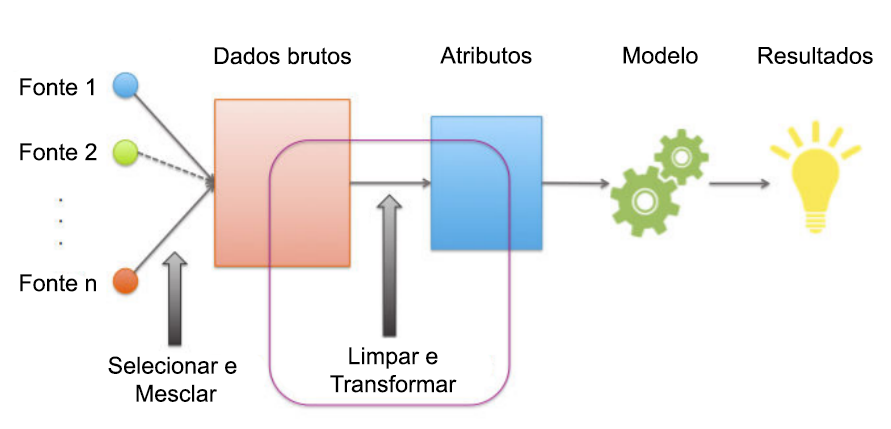
\includegraphics[width=1\textwidth]{figuras/feature-engineering.png}
        \vspace{\baselineskip} %%% linha em branco para atender a norma
        \fonte{Traduzido de \cite{book:zheng:2018}}
        \label{fig:feature-engineering}
    \end{figure}
    
    \par Como mencionado, existem inúmeras técnicas de engenharia de atributos dependendo do tipo de dados, e para cada uma delas, existem diferentes estratégias para sua aplicação. Para dados numéricos, podem ser aplicadas técnicas como: preenchimento de valores faltantes, que tem por objetivo evitar a perda de informações; arredondamento de valores, pois muitas casas decimais podem representar ruídos; transformação logarítmica, para reduzir a diferença na escala entre valores muito grandes e outros muito pequenos; normalização, para padronizar a escala dos valores; dentre outras.
    
    \par No caso de dados textuais, existem técnicas para realizar a preparação do texto, ou pré-processamento, que podem envolve alguns procedimentos como transformação em letras minúsculas, lematização das palavras, remoção de acentuações, caracteres não textuais e palavras comuns (ou \textit{stopwords}). Além disso, outros métodos de engenharia de atributos podem ser aplicados, como vetorização do texto com técnicas como \textit{bag-of-words} e \textit{word embeddings} (respectivamente bolsa de palavras e incorporação de palavras, em tradução livre), que buscam determinar a frequência e similaridade das as palavras presentes nos textos.
    
    \par Em consequência de todos os procedimentos, muitos atributos novos podem ser gerados e o processamento de todos eles pode se tornar muito custoso. Nestes casos, existem abordagens com o intuito de selecionar os atributos mais representativos dentre todos disponíveis. Dentre estas abordagens de seleção, pode-se citar Análise de Componentes Principais(PCA, do inglês: \textit{Principal Component Analysis}); método de filtragem, que busca identificar correlações entre os dados; método \textit{Wrapper} (ou de embrulhar, em tradução livre), que é baseado na tentativa e erro para encontrar a melhor combinação de atributos; e o método \textit{Embedded} (ou incorporado, em tradução livre), casos em que a seleção destes atributos já faz parte do modelo.

% % % % % % % ALGORITMOS DE APRENDIZADO DE MÁQUINA SUPERVISIONADO % % % % % % %

\section{Algoritmos de aprendizado de máquina supervisionado}
\label{sec:alg-aprend-maquina-sup}

    \par Dentro do escopo deste trabalho, que tem como um dos objetivos realizar a predição da popularidade de tuítes, requere-se a utilização da aprendizagem de máquina supervisionada, pois os resultados esperados estão diretamente ligados a classificação dos dados. Como mencionado, nesta seção serão abordados alguns dos principais algoritmos que se encaixam neste segmento e que serão utilizados no decorrer deste trabalho, apresentado suas características, funcionamento, vantagens e desvantagens na sua utilização.

% % % % % % % % NAIVE BAYES % % % % % % % %

\subsection{Naive Bayes}
\label{sec:naive-bayes}

    \par A técnica Naive Bayes pode ser considerada como uma das mais populares para classificação de dados utilizando aprendizado de máquina. O algoritmo utiliza de métodos probabilísticos, baseados na Teoria Bayesiana, criada por Thomas Bayes no século XVIII. Para compreender melhor o funcionamento dessa técnica, é importante entender também um pouco sobre o teorema do qual ela teve origem.

    \par Como mostra \cite{book:russell:10}, o teorema, ou regra de Bayes é uma formula simples, definida pela Equação \ref{eq:teorema-bayes}, que vem da regra do produto de probabilidades, assumindo que \textit{prob(D|H) = prob(H|D)}, sendo H a hipótese a ser validada e D os dados observados, podendo ser tratados também como \textit{causa} e \textit{efeito}. Apesar de simples, essa regra é a base de grande parte dos sistemas de IA (Inteligência Artificial) que utilizam inferência probabilística.
    
    \begin{equation} \label{eq:teorema-bayes}
    prob(H|D) = \frac{prob(D|H)prob(H)}{prob(D)}
    \end{equation}
    
    \par Dividindo as partes do teorema, do lado esquerdo, \textit{prob(H|D)} é chamada de probabilidade posterior da hipótese após a realização do experimento; do lado direito, \textit{prob(D|H)} chamada função de verossimilhança, é a distribuição de probabilidade dos dados, a qual multiplica-se por \textit{prob(H)}, denominada \textit{Prior}, que é a probabilidade da hipótese ser verdadeira; por fim, o denominador \textit{prob(D)}, é a probabilidade total.
    
    \par Ainda que possa parecer um teorema simples, seu alcance está na sua capacidade de interpretação. No caso do modelo Naive Bayes, ou Bayes Ingênuo, assume-se que os atributos \textit{efeito} são condicionalmente independentes entre si, dada a \textit{causa} -- daí a denominação de ``ingênuo''. A distribuição probabilística deste modelo pode ser descrita conforme indica a Equação \ref{eq:naive-bayes}, sendo \textit{C} a classe, ou causa, que deve ser prevista, enquanto que o conjunto $\{x_1, ..., x_n\}$ são os atributos, ou efeitos.
    
    \begin{equation} \label{eq:naive-bayes}
    P(C | x_1, ..., x_n) = \alpha P(C)\prod_i{P(x_i | C)}
    \end{equation}
    
    \par Este modelo de aprendizagem é facilmente escalável para problemas maiores, funcionando muito bem com uma ampla variedade de aplicações, apesar de se destacar e ser comumente utilizado em uma série algoritmos para classificação de textos. Além disso, este modelo não apresenta grandes complicações com dados ruidosos ou faltantes, podendo inclusive realizar previsões adequadas nestes casos. Esses fatores fazem o Naive Bayes ser (provavelmente) o modelo de rede Bayesiana mais comumente utilizado em algoritmos de aprendizado de máquina.
    
    \par Tomando como exemplo a clássica classificação de sentimentos em textos, como mencionado, o algoritmo irá assumir que as palavras de uma determinada mensagem não possuem uma relação entre si. Sendo assim, o classificador poderá presumir que uma frase seja positiva, caso a maioria das palavras presentes nela tenham maior probabilidade de ter este mesmo sentimento, independentemente do contexto em que foram utilizadas.
    
    \par Para classificar uma determinada frase, inicialmente é preciso montar uma base de treinamento, contendo a classificação dos dados de entrada, que no caso da análise de sentimentos, será positivo ou negativo. A partir destes dados, é criada uma tabela para guardar a frequência de cada uma das entradas com suas classes e a probabilidades de cada entrada. Para testar uma nova entrada, é calculada sua probabilidade para cada uma das possíveis classificações com base nas ocorrências anteriores. Para os casos em que o dado de teste não está presente na base de treinamento ou não foi classificado para uma das classes, existem algumas técnicas capazes de corrigir esse problema. Uma técnica muito comum aplicada para estes casos é a suavização de Laplace, a qual soma o valor 1 para todos os valores, desta forma, nenhuma operação é realizada utilizando o valor 0.
    
    \par Utilizando como exemplo a frase ``\textit{With great power comes great responsibility}'', e considerando a Tabela \ref{tab:naive-freq} (fictícia) apresentada logo abaixo, na qual consta a frequência das palavras para cada classe e a probabilidade de cada uma, para classificar a palavra ``\textit{great}'' como popular ou impopular, considerando também que essa possa ser uma frase extraída do Twitter, seriam realizadas as seguintes operações listadas a seguir.
    
    \begin{table}[ht]
        \caption{Exemplo de tabela com frequências de palavras e suas classes.}
        \centering
        \begin{tabular}{ c c c c }
            \hline
            Palavras & Popular & Impopular & Probabilidade \\
            \hline
            responsibility & 1 & 2 & 3/14 = 0,21 \\
            power & 2 & 1 & 3/14 = 0,21 \\
            great & 3 & 1 & 4/14 = 0,28 \\
            bad & 0 & 2 & 2/14 = 0,14 \\
            good & 2 & 0 & 2/14 = 0,14 \\
            \hline
            Total & 8 & 6 & \\
            \hline
            & & Positivo & 8/14 = 0,57 \\
            & & Negativo & 6/14 = 0,42 \\
            \hline
        \end{tabular}
        \vspace{\baselineskip} %%% linha em branco para atender a norma
        \fonte{Produção do próprio Autor.}
        \label{tab:naive-freq}
    \end{table}
    
    \begin{align}
    P(great|popular) = 3/8 = 0.37 \\
    P(popular) = 8/14 = 0.57 \\
    P(great) = 4/14 = 0.28 \\
    P(great|unpopular) = 1/6 = 0.16 \\
    P(unpopular) = 6/14 = 0.42
    \end{align}
    
    \begin{align}
    P(popular|great) = 0.37 * 0.57 / 0.28 = 0.75 \\
    P(unpopular|great) = 0.16 * 0.42 / 0.28 = 0.24
    \end{align}
    
    \par A partir dos cálculos realizados, com base na Tabela \ref{tab:naive-freq} apresentada, obtém-se como resultado uma probabilidade maior para a palavra `\textit{great}' ser popular. Para realizar a classificação considerando toda a frase, essa operação é aplicada para cada palavra, as probabilidades resultantes para cada classe são multiplicadas e os resultados são aplicados na regra de Bayes, conforme a Equação \ref{eq:teorema-bayes}, para cada uma das possíveis classes. Mesmo sendo um exemplo simples da aplicação da técnica Naive Bayes, é possível observar a facilidade da aplicação deste algoritmo para a classificação de dados utilizando um método probabilístico.

% % % % % % % % ÁRVORES DE DECISÃO % % % % % % % %

\subsection{Árvores de Decisão}
\label{sec:arvores-decisao}

    \par Abstraindo o conceito computacional, uma árvore de decisão pode ser definida por um fluxograma, no qual cada nó, com exceção do último nível, representa um teste sobre as informações disponíveis. O ponto de partida é denominado nó raiz. A medida que os nós filhos vão sendo explorados, as informações são divididas com o objetivo de agrupá-las por similaridade e buscando o balanceamento entre os subgrupos. Ao percorrer toda a árvore, os últimos elementos, denominados nós folha, representam a decisão a ser tomada. Apesar de ser um conceito simples, a complexidade computacional desta técnica está no processo de indução da estrutura da árvore, feita de maneira automática e não-paramétrica, podendo lidar com dados multidimensionais. 
    
    \par Assim como outras técnicas dentro do escopo de aprendizagem supervisionada, árvores de decisão também são muito populares para a resolução de problemas de classificação de dados e regressão linear. Segundo \cite{book:han:11}, a popularização deste tipo de algoritmo na aprendizagem de máquina está diretamente ligada à sua característica não-paramétrica, que permite a indução de árvores sem a o total domínio ou configuração prévia dos dados, o que torna-se muito interessante no âmbito deste trabalho no que se refere à descoberta de maneira exploratória.
    
    \par Ainda conforme \cite{book:han:11}, para realizar a classificação de dados, cada registro percorre um determinado caminho dentro da estrutura da árvore, partindo do nó raiz até o nó folha, o qual determina a classe para aquela entrada de dados. Para exemplificar, foi criada a árvore de decisão fictícia apresentada na Figura \ref{fig:exemplo_arvore}, a qual considera 4 atributos de uma mensagem de texto para considerá-la como popular ou não. Na figura, os nós com o formato retangular representam os testes feitos com cada registro de entrada, sendo que antes de cada teste é indicado o número de instâncias que estão naquele nó, partindo da raiz com 1000, já os nós com o formato circular são os nós folha, que representam a classificação final para indicar se a mensagem seria considerada como popular ou não.
    
    % IMAGEM
    \begin{figure}[!ht]
    \caption{Exemplo de árvore para classificação de um tuíte como popular.}
    \centering
    \begin{tikzpicture}
      [
        edge from parent/.style = {draw, -latex},
        every node/.style       = {font=\footnotesize},
        sibling distance        = 8em,
        level distance          = 5em,
        level 1/.style = {sibling distance=15em},
        level 2/.style = {sibling distance=8em},
        sloped,
      ]
      \node [env] {[1000] Sentimento positivo?}
        child { node [env] {[540] Maior que 140 caracteres?}
            child { node [dummy] {não} edge from parent node [above] {sim}}
            child { node [env] {[290] Possui \textit{hashtag}?}
                child { node [dummy] {não} edge from parent node [above] {sim}}
                child { node [dummy] {sim} edge from parent node [above] {não}}
                edge from parent node [above] {não}
            }
            edge from parent node [above] {sim}
        }
        child { node [env] {[460] Possui URL?}
            child { node [dummy] {sim} edge from parent node [above] {sim}}
            child { node [dummy] {não} edge from parent node [above] {não}}
            edge from parent node [above] {não}
        };
    \end{tikzpicture}
    \fonte{Produção do próprio Autor.}
    \label{fig:exemplo_arvore}
    \end{figure}
    
    \par Utilizando novamente como exemplo a frase ``\textit{With great power comes great responsibility}'', ao aplicá-la na árvore de decisão apresentada, ela seria classificada como popular, pois percorreria o seguinte caminho: Sentimento positivo; Menor que 140 caracteres; e não possui \textit{hashtag}. Uma diferença em relação a técnica \textit{Naive Bayes} que já é possível notar através deste exemplo, é que árvores de decisão são capazes de lidar com a correlação entre os atributos.
    
    \par Mesmo existindo vários algoritmos com diferentes propostas para realizar a indução de árvores de decisão, duas etapas estão presentes na grande maioria deles durante o construção da árvore, a seleção das medidas de atributos e a ``poda da árvore'' que, respectivamente, são responsáveis por definir quais a melhores partições dos dados; e por remover, ou reduzir, ruídos nas ramificações gerados durante o treinamento. Apesar de serem etapas comuns na implementação deste tipo de algoritmo, também são as etapas que os diferenciam uns dos outros dependendo da abordagem adotada para realiza-las.
    
    \par Um dos algoritmos que merece destaque por ser referência neste âmbito, é o CART (\textit{Classification and Regression Trees}), criado em 1984 por um grupo de estatísticos (L. Breiman, J. Friedman, R. Olshen, and C. Stone). Ele realiza uma abordagem de construção recursiva de divisão e conquista partindo de cima para baixo, segundo \cite{book:han:11}.


% % % % % % % % REDES NEURAIS % % % % % % % %

\begin{comment}
\subsection{Redes Neurais e Aprendizagem Profunda} % Recorrentes
\label{sec:redes-neurais}

    \par O conceito de redes neurais surgiu com o objetivo de simular o funcionamento dos neurônios do cérebro humano, capazes de realizar associações complexas em frações de segundos. Este tipo de rede funciona a partir da conexão entre nós na forma de um grafo dividido entre as camadas, que são divididas entre três tipos: camada de entrada; camada de saída; e camadas ocultas, que são todas as demais presentes entre a de entrada e de saída. 
    
    \par Apesar de ser um tópico muito popular atualmente, pesquisas envolvendo redes neurais artificiais não são tão recentes assim. Como apresentado em \cite{book:russell:10}, estudos na área de IA propondo modelos matemáticos de neurônios vem sendo realizados desde a década de 1940. De lá pra cá, segundo \citeonline{site:deep-learning}, os trabalhos neste âmbito evoluíram bastante e nos últimos anos se popularizou o uso de redes neurais de aprendizagem profunda (ou \textit{Deep Learning}), que vem sendo fundamental na implementação de sistemas inteligentes modernos, capazes de reconhecer rostos e vozes de diferentes pessoas.
    
    \par Conforme apresentado em \cite{book:russell:10}, a estrutura de uma rede neural é formada por nós matemáticos, representando neurônios, e ligações direcionadas, representando as conexões entre cada neurônio. Cada nó da rede aplica sobre sua entrada uma determinada função de ativação para gerar o valor de saída. As ligações tem o objetivo de propagar a ativação de um neurônio para o outro, sendo que cada ligação possui um determinado peso definindo força e sinal da conexão. 
    
    \par Existem diferentes funções de ativação e maneiras como a ligação entre os neurônios pode ser realizada, porém, existem duas formas para a realização destas conexões que configuram tipos de redes distintas: redes neurais com alimentação para frente (ou \textit{feed-forward}), em que suas conexões são realizadas em uma única direção, sem a presença de laços; e as Redes Neurais Recorrentes, comumente chamadas pela sigla RNN (do inglês \textit{Recurrent Neural Network}), as quais possuem laços que alimentam as entradas com suas próprias saídas, permitindo que esse tipo de rede possa armazenar memórias de curto prazo. Atualmente, a maioria dos modelos de redes profundas (\textit{deep-learning}) são totalmente baseados na estrutura de RNNs.
    
    \par Diferentemente dos primeiros modelos de redes neurais lançados, como Perceptron, os algoritmos de aprendizagem profunda modernos podem ser caracterizados por, além de recorrente, possuir várias camadas ocultas de neurônios, sendo que cada camada pode possuir diferentes tipos de função de ativação. A Figura \ref{fig:deep-learning} apresenta de forma visual a diferença na estrutura de camadas entre estes tipos de redes neurais.
    
    % IMAGEM
    \begin{figure}[ht]
        \caption{Rede Neural Simples e Rede Neural Profunda (\textit{Deep Learning})}
        \centering
        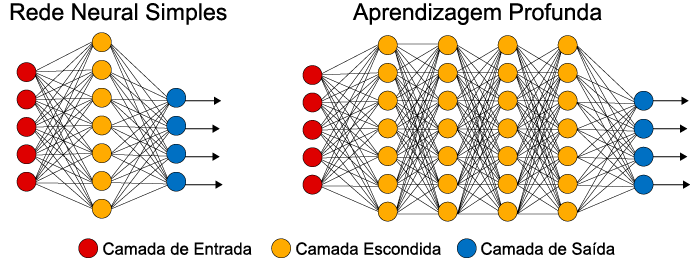
\includegraphics[width=1\textwidth]{figuras/deep-learning.png}
        \vspace{\baselineskip} %%% linha em branco para atender a norma
        \fonte{Traduzido de \citeonline{site:deep-learning}}
        \label{fig:deep-learning}
    \end{figure}
    
    \par Existem vários modelos de arquiteturas de redes neurais propostos, dentre eles, vale a pena citar: Redes Multicamadas Perceptrons; Redes de Hopfield; Redes Neurais Convolucionais; e Memória de Longo Prazo (LSTM, do inglês: \textit{Long Short-Term Memory}).
    
    % No contexto deste trabalho, durante a seção \ref{sec:experimentos}, correspondente aos experimentos, será dado destaque à arquitetura de redes convolucionais e LSTM, por se destacarem e ser muito utilizada no processamento de linguagem natural.
\end{comment}
% % % % % % % % % % % % % % % % % % % % % % % % % % % % % % % % % % % % % % 
% % % % % % % % % % % % TRABALHOS RELACIONADOS % % % % % % % % % % % % % % % 
% % % % % % % % % % % % % % % % % % % % % % % % % % % % % % % % % % % % % % 

%\chapter{Trabalhos Relacionados}
%\label{sec:trab-relacionados}

% % % % % % % % % % % % % % % % % % % % % % % % % % % % % % % % % % % % % % 
% % % % % % % % % % % % % % % % PROPOSTA % % % % % % % % % % % % % % % % % % 
% % % % % % % % % % % % % % % % % % % % % % % % % % % % % % % % % % % % % % 

\chapter{Proposta}
\label{sec:proposta}

    \par A proposta deste trabalho é a elaboração de modelos, utilizando algoritmos de aprendizado de máquina supervisionado, capaz de classificar o nível de popularidade de tuítes com base na correlação entre a taxa de engajamento dos mesmos em função de um conjunto de características presentes no corpo das mensagens e o próprio texto. Para atingir esse objetivo, é necessário coletar os tuítes, extrair suas características e aplicar os algoritmos já mencionados para realizar o treinamento e classificação dos dados. A partir disso, esta seção apresenta a definição dos atributos, definição de popularidade, arquitetura de processamento dos tuítes e os classificadores utilizados na realização do trabalho.

% % % % % % % % DEFINIÇÃO DOS ATRIBUTOS % % % % % % % %

\section{Definição dos Atributos de Interesse}
\label{sec:def-atributos}

    \par Como parte do objetivo deste trabalho é a correlação entre a popularidade e as características do texto de cada tuíte, é de fundamental importância a definição e extração de características relevantes que possam influenciar no interesse dos usuários sobre uma determinada mensagem. Esta etapa corresponde a definição dos atributos que serão extraídos de cada um dos tuítes coletados. Os itens abaixo definem cada um destes atributos e a razão de terem sido escolhidos:

    \par \textbf{Presença de URLs}: O uso de URLs em um tuíte pode indicar uma informação proveniente de outros meios, podendo ser sites de notícias ou outras mídias sociais, o que pode despertar, ou não, o interesse de usuários por um determinado tipo de informação. Esse atributo é representado pelo tipo de dados booleano, podendo ser verdadeiro ou falso.

    \par \textbf{Presença de \textit{hashtags}}: De maneira geral, as \textit{hashtags} são palavras-chave ou termos utilizados para indicar que uma determinada mensagem está diretamente ligada a um tópico ou discussão específica. O que, de maneira semelhante ao uso de URLs, pode atrair o interesse de usuários por determinados tópicos. Este atributo também é do tipo booleano.

    \par \textbf{Tamanho da mensagem}: Essa característica é basicamente a contagem da quantidade de caracteres usados no corpo do tuíte, que pode fazer com que os usuários percam o interesse em ler seu conteúdo, por ser muito curto ou muito extenso. Por tratar-se de um valor contínuo, este atributo é representado por um valor inteiro.

    \par \textbf{Sentimento da mensagem:} O sentimento é um valor que classifica o teor do texto como positivo ou negativo. Fator que pode estar diretamente ligado a intenção de cada usuário em propagar mensagens com um determinado humor. Este atributo também pode ser chamado de polaridade da mensagem e trata-se de um valor decimal, que pode variar entre -1 e 1, onde -1 corresponde a uma mensagem totalmente negativa, 0 corresponde a neutra e 1 corresponde a totalmente positiva.

    \par \textbf{Banalidade da mensagem:} No contexto deste trabalho, como também em \cite{artigo:oliveira:18}, a banalidade corresponde à importância do que foi escrito no corpo do tuíte, levando em consideração a presença de palavras que são frequentemente usadas em textos escritos na língua inglesa. Sendo assim, quanto maior o número de palavras frequentes, mais banal é a mensagem. Este atributo é representado por um valor decimal, que varia entre 0 e 1, sendo que quanto mais próximo de 1, mais banal é a mensagem. O cálculo desta métrica utiliza a Equação \ref{eq:banalidade}, apresentada logo abaixo.

    \begin{equation} \label{eq:banalidade}
    \frac{\sum_{i=1}^n (freq(P_i))}{n}
    \end{equation}
    
    \par onde o conjunto $\{P_1, ..., P_n\}$ são as palavras da mensagem após a remoção de \textit{stopwords} (preposições e artigos que normalmente são descartados durante o processamento de um texto). Já a função $freq(P)$ retorna 1 caso a palavra $P$ seja frequente e zero caso não seja.

% % % % % % % % DEFINIÇÃO DE POPULARIDADE % % % % % % % %

\section{Definição de Popularidade}
\label{sec:def-popularidade}

    \par De maneira geral, em mídias sociais, a popularidade de uma conta pode ser medida através da quantidade de seguidores que ela detém, quanto maior o número de seguidores, mais influente, ou popular, a conta é considerada. Porém, este é um indicador simples que não determina o alcance real das publicações. Para isso, existem várias métricas que permitem uma medição mais precisa sobre o impacto causado pelas ações realizadas por uma determinada página ou usuário. Uma métrica muito conhecida e utilizada para medir o alcance real de uma página sobre seus seguidores é a taxa de engajamento. Esse índice considera as interações dos fãs com os conteúdos publicados, de forma que quanto maior é essa interação, maior é o nível de engajamento.

    \par Como exposto em \cite{artigo:pillat:17}, para calcular a taxa de engajamento de uma determinada publicação, por convenção, é realizada a fórmula apresentada na Equação \ref{eq:engajamento}. Cada elemento da equação refere-se estritamente ao valor, em quantidade, obtido por cada publicação. Trazendo para a realidade do Twitter, os compartilhamentos são substituídos pelos retuítes e os comentários pelas respostas a um determinado tuíte.
    
    % EQUAÇÃO
    \begin{equation} \label{eq:engajamento}
    E(x) = \frac{curtidas + compartilhamentos + coment\acute{a}rios}{seguidores}*100
    \end{equation}
    
    \par Apesar de existir esta convenção para o cálculo do engajamento, a fórmula pode variar, dependendo das informações fornecidas por cada rede social. Como por exemplo, no caso do Facebook, o total de seguidores pode ser substituído pelo total de visualizações obtidas por cada publicação, ou então, como também apresentado em \cite{artigo:pillat:17}, substituído pelo seguidores da própria página mais os seguidores dos próprios fãs.

% % % % % % % % % % % % % % % % % % % % % % % % % % % %
% % % % % % % % % EXTRAÇÃO DOS TUÍTES % % % % % % % % %
% % % % % % % % % % % % % % % % % % % % % % % % % % % %

\section{Processamento dos Tuítes}

    \par Esta seção engloba a descrição e detalhamento dos processos envolvidos na arquitetura adotada, apresentada na Figura \ref{fig:arquitetura}, para realizar o processamento dos tuítes. Esta arquitetura, contém os seguintes módulos principais: (a) \textbf{Coleta} dos tuítes publicados por cada uma das contas acompanhadas; (b) \textbf{Extração} das características de cada tuíte; e (c) \textbf{Atualização} periódica dos dados coletados.
    
    % IMAGEM
    \begin{figure}[ht]
        \caption{Arquitetura adotada para extração de tuítes}
        \centering
        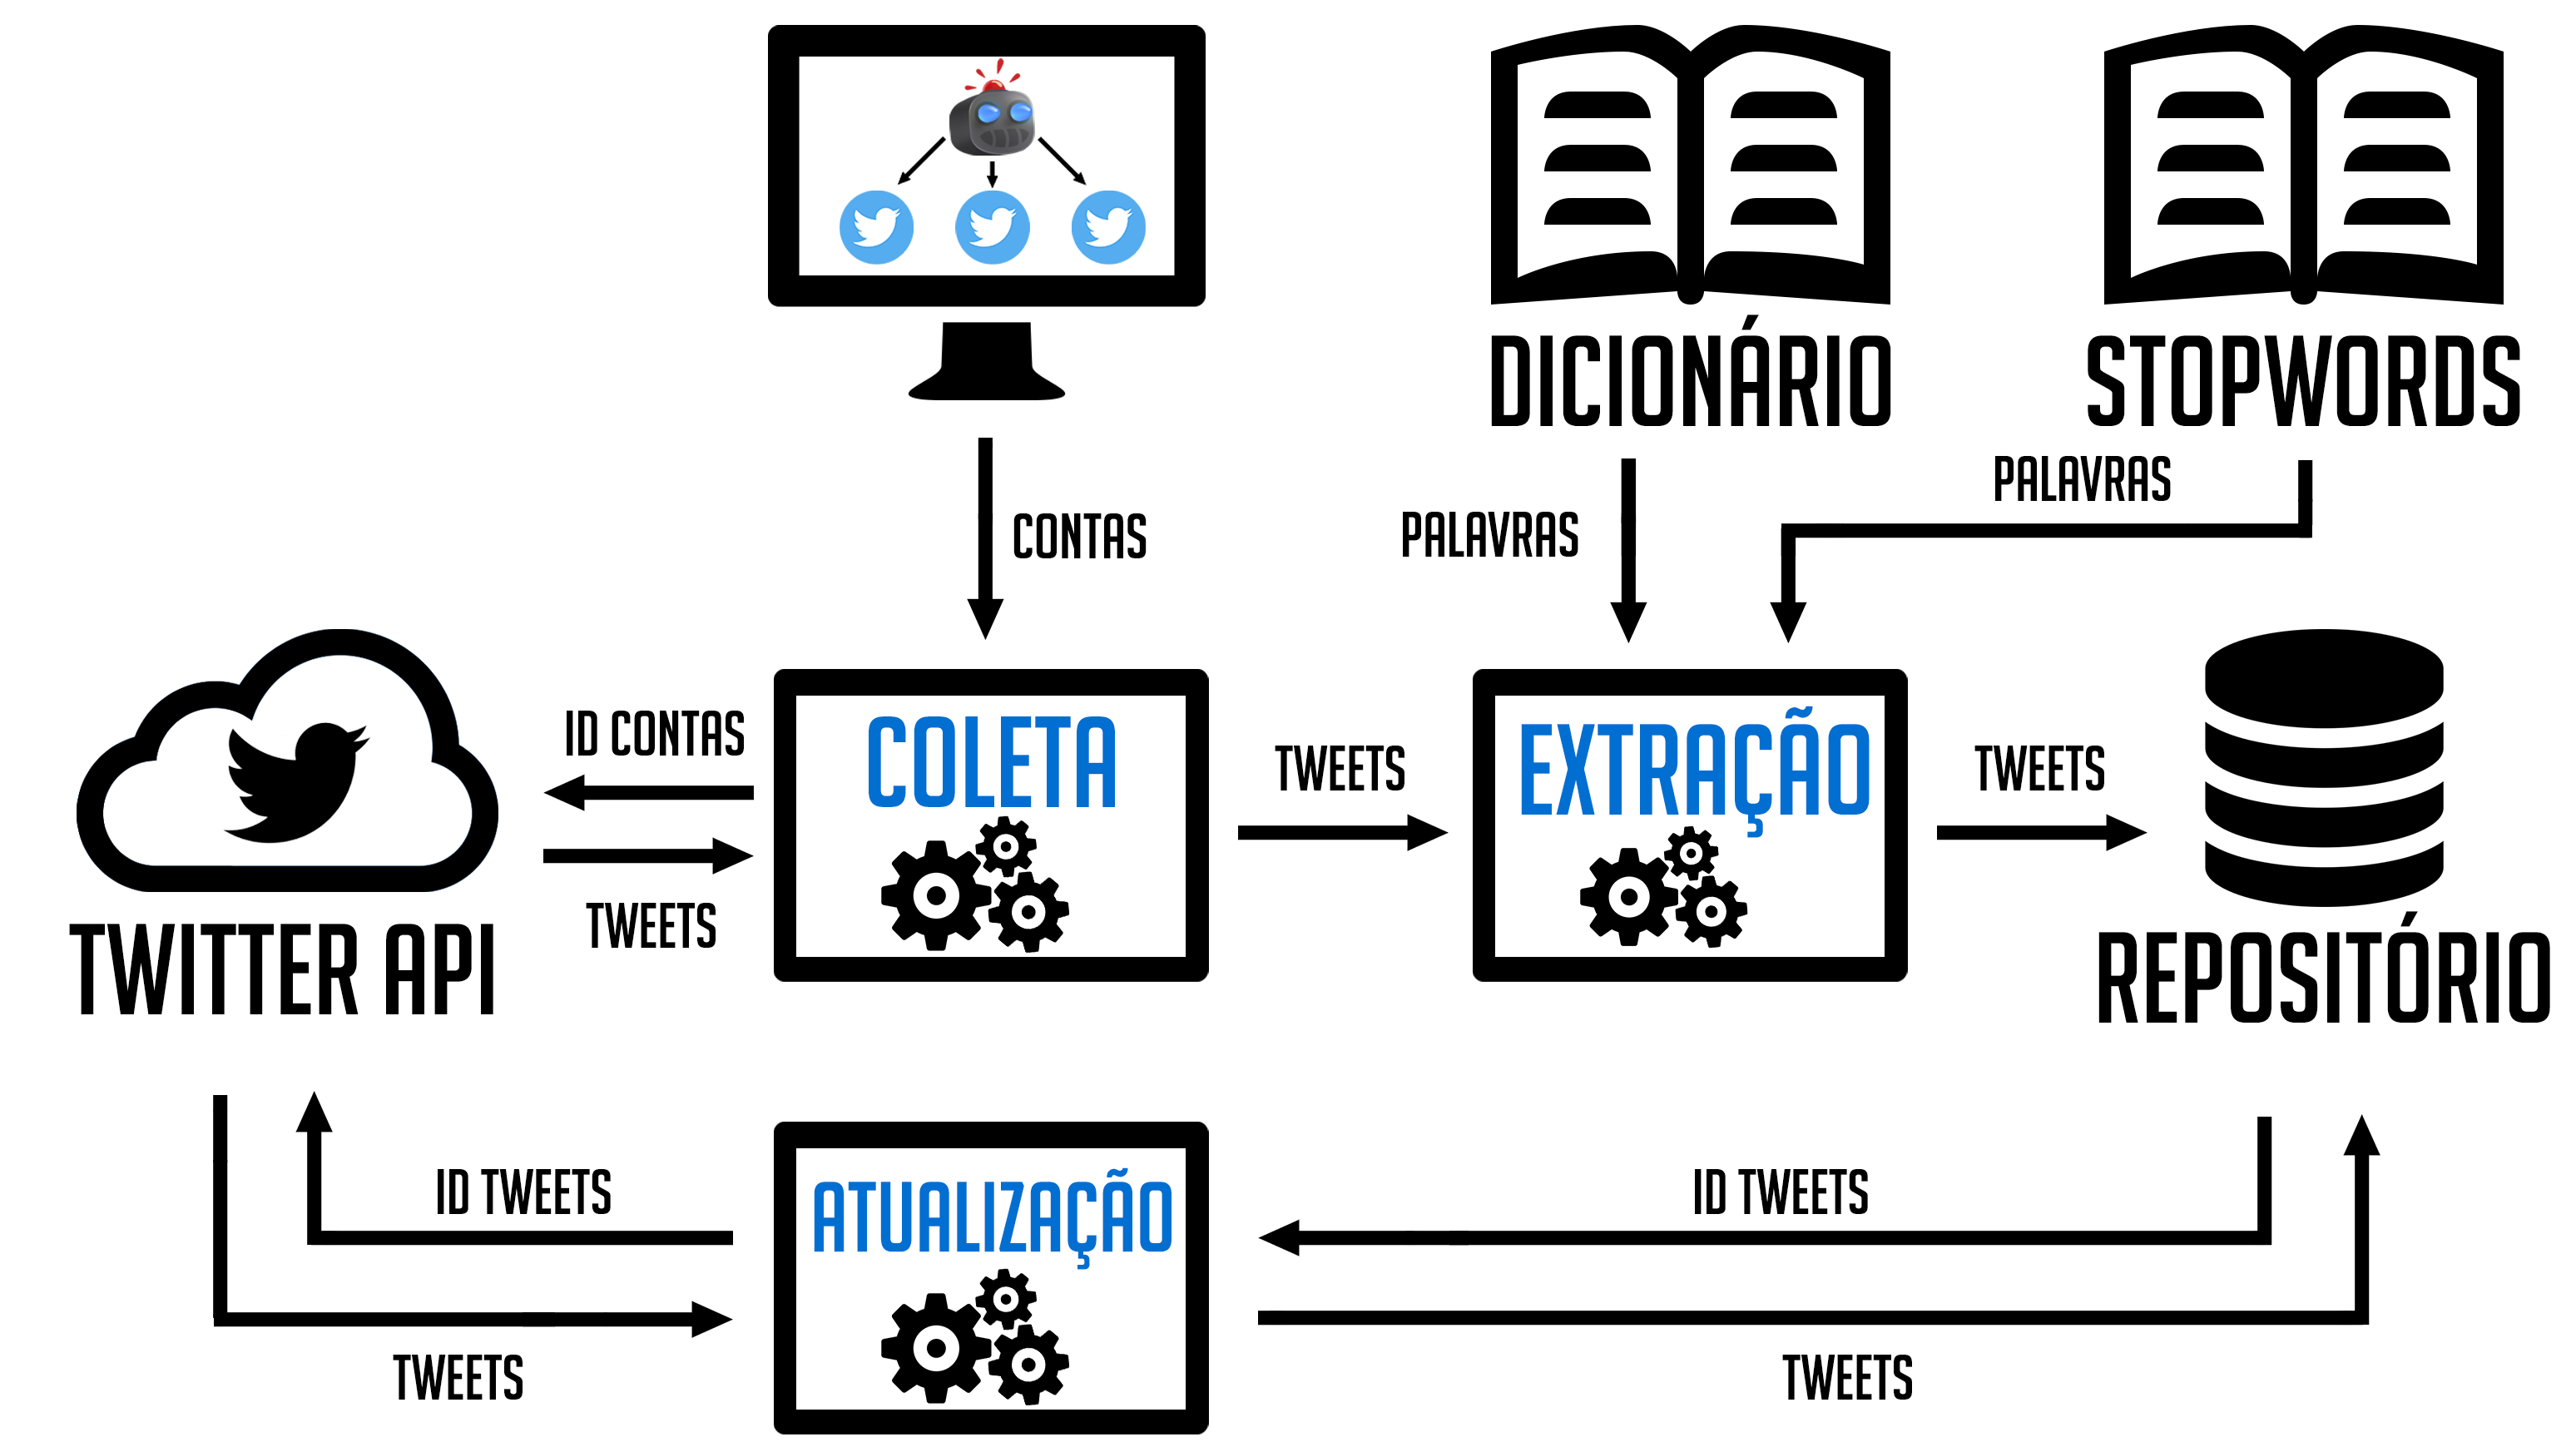
\includegraphics[width=1\textwidth]{figuras/arquitetura.png}
        \vspace{\baselineskip} %%% linha em branco para atender a norma
        \fonte{Produção do próprio autor.}
        \label{fig:arquitetura}
    \end{figure}
    
    \par A coleta dos tuítes é realizada tendo como base contas de personalidades influentes que utilizam o Twitter periodicamente. Ao todo, foram consideradas 30 contas de diversas áreas de atuação, como por exemplo Donald J. Trump (atual presidente dos Estados Unidos), Jimmy Fallon (famoso apresentador de TV americano) e Katy Perry (cantora detentora da conta com o maior número de seguidores no Twitter).
    
    \par A escolha deve-se ao fato de que a análise do impacto de publicações em redes sociais é mais relevante para esse tipo de usuário, uma vez o cálculo da taxa de engajamento para contas com poucos seguidores resultaria sempre em um valor próximo a zero. O que também é reforçado por \cite{ieee:suh:10}, quanto maior a audiência, maiores são as chances de um tuíte ser retuitado. A coleta dos tuítes foi realizada durante o ano de 2018, totalizando cerca de 9500 registros distribuídos entre as contas de interesse que foram escritos na língua inglesa.
    % período entre Novembro de 2017 e Setembro de 2018

% % % % % % % % COLETA DE TUÍTES % % % % % % % %

\subsection{Coleta dos Tuítes}

    \par O módulo de coleta é responsável por extrair tuítes de usuários específicos. A extração ocorre de forma contínua, usando recursos de \textit{streaming} disponibilizados pela API do Twitter \cite{site:twitter-api}. São coletados todos tuítes publicados a partir do momento que o \textit{streaming} entra em execução.
    
    \par A especificação das contas a serem seguidas é feita através de uma conta raiz, a partir da qual são extraídos os tuítes publicados por todos usuários seguidos por esta conta. Esta estratégia permite que novas contas sejam adicionadas à lista sem que haja interrupções na execução do algoritmo. O módulo também conta com tratamento de exceções para que a coleta não seja interrompida devido à problemas temporários de acesso aos dados, como indisponibilidade do serviço ou extrapolação do limite de requisições permitido por instante de tempo.
    
    \par Na Tabela \ref{tab:dados-coleta} podem ser visualizadas as informações extraídas de cada tuíte através da API. O campo ``mensagem'' é usado para a extração das características. Já os campos ``seguidores'', ``retuítes'' e ``curtidas'' são utilizados no cálculo para medir a taxa de engajamento de cada tuíte. Por sua vez, os campos ``identificação'' e ``data/hora'' são usados pelo módulo de atualização.
    
    % TABELA
    \begin{table}[ht]
    \centering
    \caption{Dados coletados para cada tuíte}
    \label{tab:dados-coleta}
    \begin{tabular}{|l|l|}
    \hline
    \textbf{Informação} & \textbf{Conteúdo} \\ \hline
    autor &  código e nome da conta que originou o tuíte \\ \hline
    seguidores &  quantidade de seguidores da conta que originou o tuíte \\ \hline
    identificação & código do tuíte (permite a consulta posterior) \\ \hline
    mensagem & texto de no máximo 280 caracteres \\ \hline
    data e hora & data e hora da publicação do tuíte em seu país de origem \\ \hline
    retuítes & quantidade de retuíte que a mensagem recebeu \\ \hline
    curtidas & quantidade de vezes que o tuíte foi favoritado \\ \hline
    \end{tabular}
    \end{table}
    
    \par Infelizmente a API do Twitter não permite a extração da quantidade de respostas na versão gratuita, apenas na versão para assinantes, impossibilitando a contabilização desse valor na fórmula de engajamento. Desta forma, a Equação \ref{eq:engajamento}, para o cálculo da taxa de engajamento, apresentada na seção \ref{sec:def-popularidade}, foi adaptada para considerar apenas as informações disponíveis, resultando na Equação \ref{eq:engajamento-api}.
    
    % EQUAÇÃO
    \begin{equation} \label{eq:engajamento-api}
    E(x) = \frac{curtidas + retu\acute{\imath}tes}{seguidores}*100
    \end{equation}

% % % % % % % % EXTRAÇÃO DAS CARACTERÍSTICAS % % % % % % % %

\subsection{Extração dos Atributos}

    \par Esta etapa corresponde a extração das características de cada um dos tuítes coletados. A extração ocorre imediatamente após a coleta. Os itens abaixo mostram como cada característica foi extraída:
    
    \par \textbf{Presença de URLs e \textit{hashtags}}: O uso desses recursos na mensagem é facilmente detectado pela presença de prefixos específicos no corpo da mensagem. Por exemplo, o prefixo ``http'' indica que URLs foram usadas, enquanto que o prefixo ``\#'' denota o uso de \textit{hashtags}. 
    
    \par \textbf{Tamanho da mensagem}: O tamanho é extraído através da contagem da quantidade de caracteres presentes no texto. A contagem desconsidera caracteres usados em URLs, assumindo que \textit{hiperlinks} não transmitam nenhuma mensagem.  A remoção de URLs foi realizada a partir da aplicação de uma expressão regular.

    %%%%%%%%%%%%%%% EXTRAÇÃO DO SENTIMENTO %%%%%%%%%%%%%%%
    \par \textbf{Extração do sentimento:} Para realizar a extração do sentimento, foi utilizada a biblioteca TextBlob da linguagem Python \cite{loria:14}. Essa biblioteca  permite a obtenção da polaridade e subjetividade de conteúdos textuais na língua inglesa. A API também fornece a possibilidade de tradução do conteúdo de textos escritos em outras linguagens. A extração do sentimento realizada pela biblioteca se baseia em Árvores de Decisão e no modelo de classificação \textit{Naive Bayes} -- ambos já apresentados na seção \ref{sec:fund-teorica} --, o que elimina a necessidade de elaborar no novo algoritmo para realizar essa função. 
    % assim como no trabalho de \cite{engel:16}

    %%%%%%%%%%%%%%% EXTRAÇÃO DA BANALIDADE %%%%%%%%%%%%%%%
    \par \textbf{Extração da banalidade:} A verificação da frequência utiliza um dicionário contendo 3000 palavras comuns da língua inglesa\footnote{\textit{3000 most common words in English: }\texttt{https://www.ef.com/english-resources/ english-vocabulary/top-3000-words/}}. Também são removidas as \textit{hashtags} e menções a outros usuários, por entender que não se tratam de palavras que podem ser caracterizadas como banais ou não.
    
    \par Na Tabela \ref{tab:dados-extracao} pode ser visto um exemplo geral de todas as caraterísticas extraídas nesta etapa.

    % TABELA
    \begin{table}[ht]
    \centering
    \caption{Dados obtidos na etapa de Extração}
    \label{tab:dados-extracao}
    \begin{tabular}{|l|l|}
    \hline
    \textbf{Informação} & \textbf{Conteúdo} \\ \hline
    sentimento & valor entre -1 e 1 correspondente a polaridade do texto \\ \hline
    URL & valor 1 se houver URL no texto e 0 se não houver \\ \hline
    \textit{hashtag} & valor 1 se houver \textit{hashtag} no texto e 0 se não houver \\ \hline
    tamanho & quantidade de caracteres utilizados na mensagem \\ \hline
    banalidade & somatório baseado na no uso de palavras frequentes \\ \hline
    \end{tabular}
    \end{table}


% % % % % % % % ATUALIZAÇÃO DOS DADOS % % % % % % % %

\subsection{Atualização dos Dados de Retuítes e Curtidas}

    \par Como o módulo de coleta funciona por meio de \textit{streaming}, os tuítes são coletados no instante de sua criação. Nesse momento, a quantidade de retuítes e curtidas recebidos têm o valor zero. Dessa forma, é necessária uma conferência periódica para a obtenção dos dados atualizados.
    
    \par A atualização é realizada através de um recurso da API do Twitter que obtém informações de um tuíte a partir do seu código de identificação. Para evitar sobrecarga de processamento, apenas os tuítes publicados no intervalo de 15 dias são atualizados. Como os dados de tuítes mais antigos raramente são modificados, a busca para a atualização de cada um deles seria ao mesmo tempo custosa e improdutiva.

% % % % % % % % % % % % % % % % % % % % % % % % % % % % 
% % % % % % % % CLASSIFICAÇÃO DOS TUÍTES % % % % % % % %
% % % % % % % % % % % % % % % % % % % % % % % % % % % %

\section{Classificação dos Tuítes}

    \par Esta etapa descreve os processos e ferramentas utilizados na realização da classificação dos tuítes como populares ou não populares. Para a realização da predição dos tuíte tendo como base a taxa de engajamento e considerando os atributos já mencionados, serão utilizados os algoritmos de classificação já apresentados Naive Bayes e Árvores de decisão. Os experimentos com cada algoritmo são realizados através da implementação de código utilizando a linguagem de programação Python \cite{site:python} ou com o auxilio da ferramenta Weka \cite{site:weka}.
    
    \par A utilização da linguagem Python é justificada pela grande quantidade de bibliotecas que proporcionam maior facilidade em lidar com a manipulação de dados e aprendizado de máquina. Além disso, a linguagem conquistou grande popularidade dentre a comunidade que trabalha com inteligência artificial. Dentre estas bibliotecas, uma delas merece ser destacada aqui, que é a SciKit-Learn \cite{site:scikit-learn}, que consiste em um conjunto de funcionalidades específicas para trabalhar com diferentes modelos de aprendizado de máquina, dentre elas classificação, regressão, agrupamento, redução de dimensionalidade e pré-processamento.s
    
    \par O Weka (sigla em inglês para \textit{Waikato Environment for Knowledge Analysis} e também nome de uma ave da Nova Zelândia) é uma ferramenta desenvolvida na linguagem Java que oferece um ambiente preparado para auxiliar no processo de análise e mineração de dados. Esse ambiente provê uma coleção de algoritmos capazes para realizar tarefas como preparação de dados, classificação, regressão, agrupamento, mineração de regras de associação e visualização \cite{site:weka}.

% % % % % % % % BALANCEAMENTO % % % % % % % %

\subsection{Balanceamento das instâncias}
\label{sec:class-balanceamento}
    
    \par Como apresentado em \cite{book:han:11}, a maioria dos modelos tradicionais de aprendizagem de máquina consideram que os dados de entrada já estão bem distribuídos dentre as classes, o que geralmente não acontece em bases de dados reais. Para resolver este problema, existem diversas técnicas para aperfeiçoar a classificação com dados desbalanceados, duas destas dela são: \textit{oversampling}, que consiste no preenchimento dos dados da classe com menor número até que ambas sejam equivalentes; e o \textit{undersampling}, que consiste na redução dos dados da classe com o maior número.
    
    \par Desta forma, para realizar o treinamento e a validação dos dados, independente do modelo de aprendizagem aplicado, é importante que as entradas estejam bem distribuídas entre as classes. O desbalanceamento pode resultar em um modelo tendencioso, havendo a probabilidade de classificar os dados como uma determinada classe devido à predominância da mesma no momento do treinamento.

    \par Além do balanceamento, é preciso preparar a base de dados para cada teste, isto é, configurar os dados de entrada para cada modelo considerando a taxa de engajamento e o usuário autor dos tuítes. Para realizar este processo, foi elaborado uma algoritmo que divide os registros igualmente entre as duas classes considerando uma determinada taxa de engajamento e autor passados por parâmetro. Este processo também foi escrito na linguagem Python e uma versão simplificada, em pseudo código, pode ser vista logo abaixo no algoritmo \ref{alg:get-data}.
    
    % ALGORITMO
    \begin{algorithm}[ht]
    \caption{Algoritmo para preparação dos dados}
    \label{alg:get-data}
    \begin{algorithmic}[1]
    \Function{preparaDados}{$taxa$, $autor = 0$}
        \State $tuites \gets embaralha(buscaListaDeTuites(taxa, autor))$
        \State 
        \State $max \gets maximoPorClasse(tuites)$
        \State $nPop, nNaoPop \gets 0, 0$
        \State $dados, classes \gets [ ], [ ]$
        \State
        \For{each $tw$ in $tuites$}
            \If{($nPop$ == $max$ $E$ $tw['pop']$) $OU$ ($nNaoPop$ == $max$ $E$ !$tw['pop']$)}
                \State \textit{pular}
            \EndIf
            \State 
            \State $dados.novo(tw['atributos'])$
            \State $classes.novo(tw['pop'])$
            \State
            \If{$tw['popular']$}
                \State $nPop \gets nPop + 1$
            \Else
                \State $nNaoPop \gets nNaoPop + 1$
            \EndIf
            \State
            \If{$quantidade(dados)$ == $max*2$}
                \State \textit{parar}
            \EndIf
        \EndFor
        \State \textbf{return} $dados, classes$
        \EndFunction
    \end{algorithmic}
    \end{algorithm}
    
    \par O algoritmo tem como entrada a taxa de engajamento e o código do autor, que pode não ser informado, para o caso de análises gerais. Como primeira instrução, é feita uma busca pelos tuítes considerando a taxa e o usuário. A própria função de busca faz o tratamento da necessidade de distinção dos dados por usuário. Tento a lista completa, é identificada a classe que possui o menor número de registros, sendo esta a variável responsável pelo balanceamento. São inicializadas as variáveis de controle (\textit{nPop} e \textit{nNaoPop}), \textit{dados} e \textit{classes}. Em seguida é feito um laço de repetição para cada tuíte. Para cada iteração do laço é feita uma verificação da quantidade de entradas em cada classe através das variáveis de controle e, se o valor for menor que o máximo, os atributos e classe são guardados. Por fim, as variáveis de controle são incrementadas. O laço termina quando a quantidade de dados alcança o valor máximo, retornando então as listas balanceados.
    
    \par O código descrito no Algoritmo \ref{alg:get-data} é uma versão reduzida. Há ainda o trecho responsável pela geração do arquivo para utilização no Weka, se necessário for. O formato deste arquivo gerado pelo código e aceito pela ferramenta é o ARFF (sigla em inglês para \textit{Attribute-Relation File Format}).

% % % % % % CLASSIFICAÇÃO COM NAIVE BAYES E ÁRVORES DE DECISAO % % % % % %

\subsection{Classificação utilizando Naive Bayes e Árvores de Decisão}
\label{sec:class-naive-tree}

    \par Como já mencionado, a classificação dos dados será realizada utilizando os algoritmos Naive Bayes e Árvores de Decisão. No caso do modelo de Bayes para classificação binária, os experimentos são realizados em duas vertentes, sendo uma delas a aplicação do algoritmo utilizando somente o texto pré-processado dos tuítes e a outra utilizando os atributos coletados.
    
    \par O modelo Naive Bayes utilizando texto foi implementado utilizando a linguagem Python, com o auxílio da biblioteca para aprendizado de máquina Scikit-Learn. O algoritmo é baseado em cálculos probabilísticos conforme apresentado na seção \ref{sec:naive-bayes} e, assim como código de balanceamento apresentado, este também recebe como parâmetros de entrada a taxa de engajamento e o usuário autor. Ao final da execução, como retorno são apresentadas as métricas de avaliação do modelo, juntamente com a matriz de confusão. Esse formato de saída foi adotado com o objetivo de manter a consistência com os resultados obtidos a partir dos testes uilizando o Weka.
    
    \par No caso dos experimentos utilizando os atributos coletados, tando a segunda opção do Naive Bayes quanto as Árvores de Decisão, estes serão realizados utilizando o Weka, devido sua praticidade em realizar o treinamento e validação dos dados a partir do arquivo gerado. Quanto aos modelos de árvores, os testes serão realizados focando nos algoritmos J48  e LTM (sigla para \textit{Logistic Model Trees}).


% % % % % % % % % % % % % % % % % % % % % % % % % % % % % % % % % % % % % % 
% % % % % % % % % % % % % % METODOLOGIA  % % % % % % % % % % % % % % % % % 
% % % % % % % % % % % % % % % % % % % % % % % % % % % % % % % % % % % % % % 

\begin{comment}
\chapter{Metodologia}
\label{sec:metodologia}

    \par Para alcançar os objetivos elencados, uma série de etapas foi elaborada para a realização deste projeto, nas quais o sucesso de uma está diretamente ligado ao da outra. A fim de proporcionar maior compreensão destas etapas, este capítulo foi destinado à descrição de cada uma destas etapas juntamente com a apresentação do cronograma do projeto, no qual consta a previsão de realização de cada uma delas.
    
    \par \textbf{Análise de trabalhos similares:} Nesta etapa será realizada uma pesquisa sobre trabalhos similares já realizados na área envolvendo aprendizado de máquina e extração de dados extraídos do Twitter, com o objetivo de que os mesmos possam vir a auxiliar e contribuir com a proposta do trabalho.
    
    \par \textbf{Definição dos atributos:} Esta etapa é designada para analisar e definir quais serão os atributos de interesse que devem ser extraídos de cada tuíte, considerando a relevância que cada um deles pode inferir sobre a popularidade daquele tuíte.
    
    \par \textbf{Extração e pré-processamento dos dados:} Dispondo dos atributos de interesse, os tuítes devem ser coletados e seus conteúdos pré-processados. Para isso, será realizado um estudo acerca dos melhores métodos e ferramentas que permitem a extração de dados do Twitter e posteriormente de seus atributos de interesse.
    
    \par \textbf{Estudo de algoritmos de aprendizado de máquina:} Estando em posse dos dados já processados, será realizado um estudo acerca dos algoritmos de aprendizado de máquina para classificação de dados e quais são as melhores opções considerando os dados de entrada e os atributos de interesse.
    
    \par \textbf{Implementação dos algoritmos:} Dispondo do conhecimento necessário acerca algoritmos de aprendizado de máquina e os atributos disponíveis, serão implementados tais algoritmos utilizando tecnologias adequadas para tal.
    
    \par \textbf{Experimentos com os algoritmos selecionados:} Esta etapa corresponde a realização de testes com os algoritmos estudados e implementados nas etapas anteriore. O experimentos serão realizados com o objetivo de classificar a popularidade dos tuítes com base nos atributos extraídos.
    
    \par \textbf{Análise dos resultados obtidos:} Esta etapa do trabalho destina-se a realização de uma análise sobre os algoritmos testados e os resultados obtidos com cada um deles ao tentar realizar a predição da popularidade dos tuítes.
    
    \par \textbf{Documentação:} Por fim, é nesta etapa que os resultados obtidos com o decorrer do projeto são analisados e documentados, havendo a chance de originar um artigo, considerando que houve certa contribuição científica com a área, além do próprio relatório do Trabalho de Conclusão de Curso.
    
    \section{Cronograma}
    
    \par Com base nas etapas descritas, a Tabela \ref{tab:cronograma} a seguir resume o cronograma das atividades previstas. Dividido entre quinzenas, o cronograma tem início a partir do mês de Agosto (08). As atividades já realizadas até o momento compreendem os itens marcados com bola ($\bullet$) e fundo em cinza, enquanto que os marcadores em xis ($\times$) com fundo branco representam as atividades que ainda devem ser realizadas.
    
    \begin{table}[ht]
    \centering
    \caption{Cronograma do projeto}
    \label{tab:cronograma}
    \begin{tabular}{|l|c|c|c|c|c|c|c|c|}
    \hline
    \textbf{Atividade} & \textbf{8/2} & \textbf{9/1} & \textbf{9/2} & \textbf{10/1} & \textbf{10/2} & \textbf{11/1} & \textbf{11/2} & \textbf{12/1} \\ \hline
    Análise de trabalhos similares & \cellcolor{gray!20}$\bullet$ & \cellcolor{gray!20}$\bullet$  &  &  &  &  &  &  \\ \hline
    Definição dos Atributos & \cellcolor{gray!20}$\bullet$ & \cellcolor{gray!20}$\bullet$ & \cellcolor{gray!20}$\bullet$ &  &  &  &  &  \\ \hline
    Extração e pré-processamento &  & \cellcolor{gray!20}$\bullet$ & \cellcolor{gray!20}$\bullet$ & \cellcolor{gray!20}$\bullet$ & \cellcolor{gray!20}$\bullet$ &  &  &  \\ \hline
    Estudo de algoritmos de IA &  &  &  & \cellcolor{gray!20}$\bullet$ & \cellcolor{gray!20}$\bullet$ & \cellcolor{gray!20}$\bullet$ &  &  \\ \hline
    Implementação dos algoritmos &  &  &  & \cellcolor{gray!20}$\bullet$ & \cellcolor{gray!20}$\bullet$ & $\times$ & $\times$ & $\times$ \\ \hline
    Experimentos com algoritmos &  &  &  & \cellcolor{gray!20}$\bullet$ & \cellcolor{gray!20}$\bullet$ & $\times$ & $\times$ & $\times$ \\ \hline
    Análise dos resultados obtidos &  &  &  &  &  & $\times$ & $\times$ & $\times$ \\ \hline
    Documentação & \cellcolor{gray!20}$\bullet$ & \cellcolor{gray!20}$\bullet$ & \cellcolor{gray!20}$\bullet$ & \cellcolor{gray!20}$\bullet$ & \cellcolor{gray!20}$\bullet$ & $\times$ & $\times$ & $\times$ \\ \hline
    \end{tabular}
    \end{table}
\end{comment}

% % % % % % % % % % % % % % % % % % % % % % % % % % % % % % % % % % % % % % 
% % % % % % % % % % % % % % EXPERIMENTOS  % % % % % % % % % % % % % % % % % 
% % % % % % % % % % % % % % % % % % % % % % % % % % % % % % % % % % % % % % 

\chapter{Experimentos}
\label{sec:experimentos}

    \par Com base nos fundamentos e proposta apresentados, respectivamente nas seções \ref{sec:fund-teorica} e \ref{sec:proposta}, neste capítulo serão apresentados os experimentos realizados e resultados obtidos com a aplicação dos algoritmos sugeridos sobre os dados coletados. De maneira geral, os experimentos tem por objetivo realizar análises sobre a aplicação dos algoritmos de aprendizado de máquina, variando o usuário e a taxa de engajamento para determinar a popularidade. O intuito é identificar uma possível correlação entre estas variantes e as características extraídas de cada tuítes.
    
% % % % % % % % MÉTRICAS % % % % % % % %

\section{Métricas de Avaliação}
\label{sec:class-metricas}

    \par Para poder realizar a avaliação dos modelos de avaliação, é importante definir as métricas que serão utilizadas para realizar essa comparação entre os modelos. Para isso, serão consideradas cinco métricas, sendo acurácia, sensibilidade, especificidade, valor preditivo positivo e valor preditivo negativo. Estas medidas, apresentadas nas equações \ref{eq:acuracidade}, \ref{eq:sensibilidade}, \ref{eq:especificidade}, \ref{eq:predit-neg} e \ref{eq:predit-neg}, retiradas de \cite{book:han:11}, são aplicadas após a etapa de validação e consideram os acertos e erros dos algoritmos sobre cada uma das classes em relação ao total de cada classe.
    
    % EQUAÇÃO
    \begin{equation} \label{eq:acuracidade}
    Acur\acute{a}cia = \frac{AcertosPositivos + AcertosNegativos}{TotalPositivos + TotalNegativos}
    \end{equation}
    
    % EQUAÇÃO
    \begin{equation} \label{eq:sensibilidade}
    Sensibilidade = \frac{AcertosPositivos}{TotalPositivos}
    \end{equation}
    
    % EQUAÇÃO
    \begin{equation} \label{eq:especificidade}
    Especificidade = \frac{AcertosNegativos}{TotalNegativos}
    \end{equation}
    
    % EQUAÇÃO
    \begin{equation} \label{eq:predit-pos}
    PreditivoPositivo = \frac{AcertosPositivos}{AcertosPositivos + FalsosPositivos}
    \end{equation}
    
    % EQUAÇÃO
    \begin{equation} \label{eq:predit-neg}
    PreditivoNegativo = \frac{AcertosNegativos}{AcertosNegativos + FalsosNegativos}
    \end{equation}
    
    \par A acuracidade é uma medida de análise geral dos acertos, sem diferenciar as classes. Enquanto que a Sensibilidade e a Especificidade são as medidas que indicam a capacidade do modelo em realizar a predição das entradas como a classe positiva e negativa, respectivamente. Já os valores preditivos, estão relacionados com o total de predições corretas de uma das classes com o total de predições realizadas. 
    
% % % % % % % % APLICAÇÃO DOS CLASSIFICADORES % % % % % % % %

\section{Aplicação dos classificadores}
\label{sec:exp-class}

    \par Apresentação dos gráficos e descrição dos resultados.
    
    % DADOS
    \pgfplotstableread[row sep=\\,col sep=&]{
        algorithm       & tx010 & tx020  & tx030 & tx040 & tx100 & tx200 \\
        NBayesTexto     & 0.658 & 0.681  & 0.670 & 0.662 & 0.674 & 0.679 \\
        NBayesAtributos & 0.631 & 0.617  & 0.610 & 0.603 & 0.564 & 0.606 \\
        J48             & 0.637 & 0.619  & 0.607 & 0.604 & 0.579 & 0.651 \\
        LMT             & 0.634 & 0.615  & 0.609 & 0.598 & 0.596 & 0.641 \\
        }\mydata
    
    % GRÁFICO
    \begin{figure}[!ht]
    \caption{Acurácia de cada algoritmo aplicado sobre toda a base com diferentes taxas de engajamento.}
    \centering
    \begin{tikzpicture}
        \begin{axis}[
                ybar,
                enlarge x limits={abs=1.75cm},
                bar width=0.42cm,
                width=\textwidth,
                height=.5\textwidth,
                legend style={at={(0.5,1)},
                    anchor=north,legend columns=-1},
                symbolic x coords={NBayesTexto, NBayesAtributos, J48, LMT},
                xtick=data,
                %nodes near coords,
                %nodes near coords align={vertical},
                ymin=0.55,ymax=0.71,
                ylabel={acurácia},
                legend image code/.code={%
                   \draw[#1, draw=none] (0cm,-0.2cm) rectangle (0.44cm,0.2cm);
                },
            ]
            \addplot [fill=myblue!75,postaction={pattern=north east lines, pattern color=Blue}] table[x=algorithm,y=tx010]{\mydata};
            
            \addplot [fill=myred!70,postaction={pattern=horizontal lines, pattern color=Mahogany}] table[x=algorithm,y=tx020]{\mydata};
            
            \addplot [fill=YellowOrange,postaction={pattern=vertical lines, pattern color=Yellow}] table[x=algorithm,y=tx030]{\mydata};
            
            \addplot [fill=ForestGreen,postaction={pattern=north east lines, pattern color=SkyBlue}] table[x=algorithm,y=tx040]{\mydata};
            
            \addplot [fill=Orange,postaction={pattern=dots, pattern color=Goldenrod}] table[x=algorithm,y=tx100]{\mydata};
            
            \addplot [fill=Aquamarine,postaction={pattern=horizontal lines, pattern color=white}] table[x=algorithm,y=tx200]{\mydata};
            
            \legend{1.0\%, 2.0\%, 3.0\%, 4.0\%, 10.0\%, 20.0\%}
        \end{axis}
    \end{tikzpicture}
    \fonte{Produção do próprio autor.}
    \label{fig:analise-geral}
    \end{figure}
    
    \begin{figure}[!ht]
    \caption{Variação no número de instâncias balanceadas por taxa de engajamento.}
    \centering
    \begin{tikzpicture}
        \begin{axis}[
            width=\textwidth,
            height=.5\textwidth,
            symbolic x coords={1.0\%, 2.0\%, 3.0\%, 4.0\%, 10.0\%, 20.0\%},
            xtick=data,
        ]
            
            \addplot[mark=triangle*, mark size=4, draw=myblue,  mark options={solid}, myblue, thick, dashed] coordinates {
                (1.0\%, 0.727) (2.0\%, 1.000) (3.0\%, 0.772) (4.0\%, 0.715) (10.0\%, 0.394) (20.0\%, 0.187)
            }node[pos=0.7,above,anchor=east]{Balanceamento};
            
        \end{axis}
    \end{tikzpicture}
    \fonte{Produção do próprio autor.}
    \label{fig:engaj-balanc}
    \end{figure}

    \begin{figure}[!ht]
    \caption{Variação no número de instâncias em relação às métricas para o algoritmo Naive Bayes utilizando o texto.}
    \centering
    \begin{tikzpicture}
        \begin{axis}[
            width=\textwidth,
            symbolic x coords={1.0\%, 2.0\%, 3.0\%, 4.0\%, 10.0\%, 20.0\%},
            xtick=data,
            %ymin=0.55,ymax=0.71,
        ]
            
            \addplot[mark=triangle*, mark size=4, draw=myblue,  mark options={solid}, myblue, thick, dashed] coordinates {
                (1.0\%, 0.727) (2.0\%, 1.000) (3.0\%, 0.772) (4.0\%, 0.715) (10.0\%, 0.394) (20.0\%, 0.187)
            }node[pos=0.3,above,anchor=south west]{Balanceamento};
            
            \addplot[mark=diamond*, mark size=5, draw=myred, thick, myred] coordinates { 
                (1.0\%, 0.658) (2.0\%, 0.681) (3.0\%, 0.670) (4.0\%, 0.662) (10.0\%, 0.674) (20.0\%, 0.679)
            }node[pos=0.7,above,anchor=north west]{Acurácia};
            
            \addplot[mark=square*, mark size=3, draw=ForestGreen, thick, ForestGreen] coordinates { 
                (1.0\%, 0.742) (2.0\%, 0.764) (3.0\%, 0.789) (4.0\%, 0.784) (10.0\%, 0.867) (20.0\%, 0.885)
            }node[pos=0.7,above,anchor=north west]{Sensibilidade};
            
            \addplot[mark=*, mark size=4, draw=YellowOrange, thick, YellowOrange] coordinates { 
                (1.0\%, 0.577) (2.0\%, 0.599) (3.0\%, 0.551) (4.0\%, 0.539) (10.0\%, 0.487) (20.0\%, 0.474)
            }node[pos=0.4,above,anchor=north]{Especificidade};
        \end{axis}
    \end{tikzpicture}
    \fonte{Produção do próprio autor.}
    \label{fig:balanc-metricas}
    \end{figure}

% % % % % % % % % % % % % % % % % % % % % % % % % % % % % % % % % % % % % % 
% % % % % % % % % % % % % % % CONCLUSÕES % % % % % % % % % % % % % % % % % %
% % % % % % % % % % % % % % % % % % % % % % % % % % % % % % % % % % % % % % 

\chapter{Conclusões}
\label{sec:conclusao}

    \par Considerações finais e trabalhos futuros.

% % % % % % % % % % % % % % % % % % % % % % % % % % % % % % % % % % % % % % 
% % % % % % % % % % % % FIM DAS PAGINAS TEXTUAIS % % % % % % % % % % % % % % 
% % % % % % % % % % % % % % % % % % % % % % % % % % % % % % % % % % % % % % 


% % % % % % % % % % % % % % % % % % % % % % % % % % % % % % % % % % % % % % 	
% % % % % % % % % % % % % BIBLIOGRAFIA  % % % % % % % % % % % % % % % % % % 
% % % % % % % % % % % % % % % % % % % % % % % % % % % % % % % % % % % % % % 	

\bibliografia{referencias}  %%%%% BIBLIOGRAFIA -> NOME DO ARQUIVO *.BIB	
	
% % % % % % % % % % % % % % % % % % % % % % % % % % % % % % % % % % % % % 	
% % % % % % % % % % % % % APÊNDICES % % % % % % % % % % % % % % % % % % %
% % % % % % % % % % % % % % % % % % % % % % % % % % % % % % % % % % % % % 	
\apendice %%%% TEXTOS A PARIR DESTE PONTO SERÃO CONSIDERADOS APÊNDICES

    %\chapter{Demonstração de algo}
    %\label{sec:apendice-demonst-algo}
            %\par Algo como apêndice.  
        
% % % % % % % % % % % % % % % % % % % % % % % % % % % % % % % % % % % % % % 	
% % % % % % % % % % % % % % % ANEXOS  % % % % % % % % % % % % % % % % % % % 
% % % % % % % % % % % % % % % % % % % % % % % % % % % % % % % % % % % % % % 	
\anexo    %%%% TEXTOS A PARIR DESTE PONTO SERÃO CONSIDERADOS ANEXOS

    %\chapter{Algo interessante que alguém fez}
    %\label{sec:anexo-algo-interessante}
             %\par Algo como anexo.

\end{document}

